\documentclass[a4paper, 12pt]{article}
\usepackage{ amssymb, amsmath}

\usepackage[latin1]{inputenc}

\usepackage{theorem}

\usepackage[pdftex]{graphicx}
\usepackage{url}
\usepackage{dsfont}

\usepackage[parfill]{parskip}
\usepackage{tabularx, calc}

\newenvironment{tipp}{\noindent{\bf Tip: }\itshape}{\par}
\newenvironment{hinweis}{\noindent{\bf Note: }\itshape}{\par}
\newenvironment{beispiel}{\noindent{\bf Example: }\itshape}{\par}


\newcommand{\tweak}{\hspace*{1.5pt}}
\newcommand{\gf}[1]{``{#1}''}

%\parindent 0pt
%\parskip 6pt

\setcounter{secnumdepth}{2}
%\setcounter{tocdepth}{1}

\newlength\myheight
\newlength\mydepth
\settototalheight\myheight{Xygp}
\settodepth\mydepth{Xygp}
\setlength\fboxsep{0pt}
\newcommand*\inlinegraphics[1]{%
  \settototalheight\myheight{Xygp}%
  \settodepth\mydepth{Xygp}%
%  \raisebox{-\mydepth}{\includegraphics[height=\myheight]{#1}}%
 \raisebox{-\mydepth}{\includegraphics{#1}}% 
}

\usepackage{wrapfig}

\usepackage[colorlinks,
pdfpagelabels,
pdfstartview = FitH,
bookmarksopen = true,
bookmarksnumbered = true,
linkcolor = blue,
plainpages = false,
hypertexnames = false,
citecolor = black] {hyperref}

\usepackage[a4paper,left=2.6cm, right=2.9cm,top=2.5cm, bottom=2.5cm]{geometry}


\begin{document}

\begin{titlepage}
	\centering
	{\scshape\LARGE Nemp - Noch ein mp3-Player\footnote{\emph{Noch ein mp3-Player} translates to \emph{Yet another mp3-player}} \par}
	
	Version 4.12 \par
	\vspace{1cm}
	
\includegraphics[width=0.5\textwidth]{nemp.jpg}\par
	\vspace{1cm}
	{\Large Documentation and user guide\par}	
	\emph{This documentation was mainly translated with the help of \emph{deepl.com}. I hope it is reasonably understandable and does not contain too much gibberish.}	
	\vfill	
	\copyright Daniel Gau�mann, 2005-2019
\end{titlepage}

\tableofcontents

\newpage

\section{Nemp Basics}

The Player Nemp was developed out of my own needs. I didn't find any player\footnote{actually: no \emph{program}, because an \emph{player} was originally not planned... } which fulfilled my requirements. So I just sat down and started programming. Over time, more and more features have been added, much of it through feedback from a small group of people using the player.

I have always tried to keep the basic handling as simple as possible.

\subsection{Basic Settings: The Nemp Wizard}
\label{sec_wizard}

At the first start the Nemp Wizard is started, which provides some basic configurations. You can also skip these settings and repeat them later.


\begin{wrapfigure}{R}{0.21\textwidth}
\centering

\includegraphics[width=0.2\textwidth]{wizard.png}
\end{wrapfigure}
Nemp has a lot of interesting features. Some of them are very useful (at least I think so), but some of them change your music files, or look for additional information on the Internet.

I think that such things should be \textbf{Opt-in}. I don't like players that write stuff into my ID3 tags without asking. I don't like programs that go online all by themselves to do something. Therefore, the Nemp Wizard was introduced, which asks some basic questions at the first start of Nemp. 

For the following actions, the Nemp Wizard will ask for permission:

\begin{itemize}
\item Check for updates: Nemp will download a small text file from my website www.gausi.de to point out a newer version if one exists. This happens once a week in the standard setting, but can also happen more often. No personal data is sent, and apart from the usual server logs (IP-address etc.) I don't get anything else from it. I don't care, either.

\item Change metadata: Nemp uses the metadata (ID3 tags) of the audio files to store various information. Changing this data is very easy - just click on it to change the rating - and could happen unintentionally. But this is a common feature, and many other players just do it as well. 

\item Automatic rating: Nemp can automatically adjust the rating of your music files. If you listen to a song often, it is likely that you like it. If you break it off, it is probably not that great. The rating is also written to the metadata of the file. 

\item Download missing covers: If no suitable cover for a music file can be found on the hard disk, Nemp can try to download a cover from the internet via the last.fm web service. This is then stored in the Nemp cover folder, and as \texttt{NempAutoCover.jpg} (or \texttt{.png}) in the directory where the music file itself is located. 

\item Nemp as default player: Register Nemp as the default player for Windows. Under Windows 10 this doesn't  work 100\% - Windows will probably ask you again with which \emph{App} you want to open an mp3-file.
\end{itemize}

If you cancel the wizard at some point, all of these options will remain unchanged - i.e. deactivated in the default setting.

You can change these settings later by restarting the wizard from the menu or using the full \hyperref[sec_einstellungen]{Settings dialog}. 


%And just to start now: Click the Play button, select a few files in the selection dialog and listen to some music while reading this documentation.

%\begin{center}
%
\includegraphics{BtnPlay.png} 
%\end{center}

\subsection{Filling the Playlist and creating the Media Library}
%\subsubsection{Der Player}

When you have finished the setting wizard, you can start playing music. The main window of Nemp consists of several parts. At the beginning, i.e. when the playlist and media library are empty, some hints are visible to make the start a little easier.

\begin{figure}[htb]
\centering
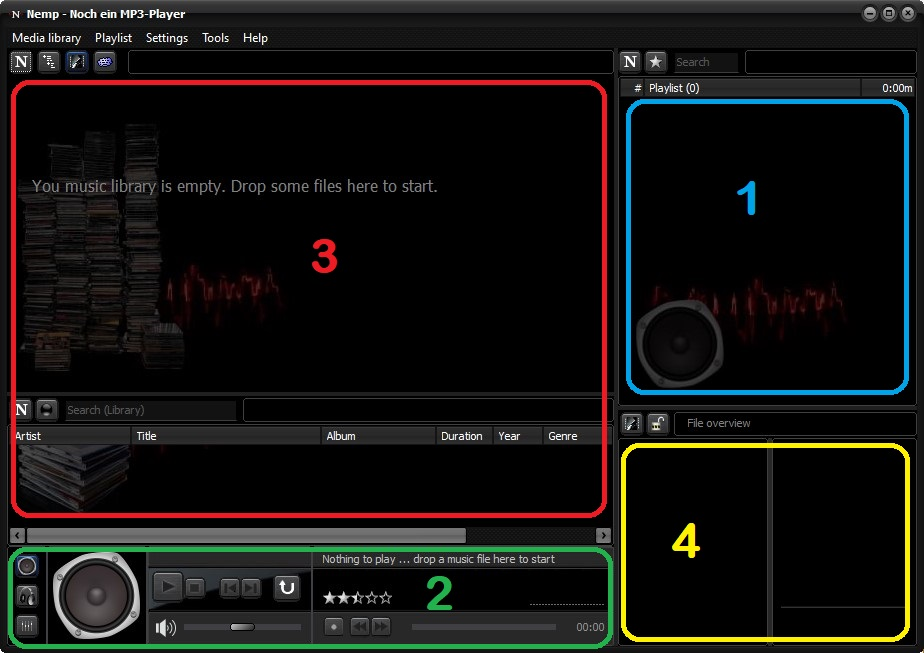
\includegraphics[width=0.8\textwidth]{Nemp1stStart.jpg}
\label{fig_hauptfenster}
\end{figure}

The arrangement of the individual areas can be configured since version 4.11, more on this later. The default setting is the same as in this picture.

\subsubsection{Playing music}

To start playing music, you can simply drag a few music files (or a folder) to the player or playlist area. This is the part at the bottom left with the usual controls, or the large area at the top right. Nemp will then start playing automatically.

Alternatively, you can click on the Play button. Then a dialog for the selection of music files opens. And of course it can be done extra-complicated via the menu: Playlist $\rightarrow$ Add files, add directory, load playlist, whatever. Or you use Copy\& Paste (\texttt{Ctrl+C, Ctrl+V}) from Windows Explorer. 

\subsubsection{Creating the Media Library}

An essential part of Nemp is the \emph{media library}. There all music files are managed. You can then browse your music collection according to different criteria or search for individual titles.

To build up the media library simply drag your main music folder into the given area. Searching the hard disk and reading the metadata takes a little time. But this only has to be done once, then the data is saved and is (almost) immediately available the next time you start Nemp.

\subsubsection{Title information}

When you highlight a title in the media library or playlist, some information about that title is displayed in the \emph{File Information} area. Beside the cover picture or the lyrics some more (title, artist, album, genre, year, as well as \gf{extended tags}).

About this part is also some browsing in the media library possible, as well as the creation of \gf{additional tags}. Read more in the \hyperref[sec_titleinformation]{Browse the Media Library} section.


\subsection{Basic control}


During the development of Nemp I tried to offer as many possibilities for control as possible, which are common under Windows. These include:

\begin{itemize}
\item Clicking on buttons.
\item Tabbing through the controls with the \texttt{Tab} key and activating the focused element with \texttt{Enter}.
\item Context menus. The four areas (partly also some individual elements) have their own context menu, which can be used to call various functions. You can access the context menu by right-clicking on the right mouse button or by clicking on one of the Nemp buttons. 
\includegraphics{TabBtnNemp.png}
\item Shortcut keys such as \texttt{Ctrl+F} for quick search or \texttt{Ctrl+D} for displaying details of a selected title.
\item The usual Windows methods \emph{Drag\&Drop} and \emph{Copy\&Paste} are available for handling files. If Nemp is the target of such an operation, a distinction is made between playlist and media library. A \emph{dropped} folder is either inserted into the playlist or into the media library. If you want to insert music files into other programs from within Nemp, this is limited to 2500 files for performance reasons.
\item Multimedia keyboards are also supported. Pressing one of these special keys should also effect the desired action in Nemp.
\item Optionally global hotkeys can be defined, e.g. \texttt{Ctrl+Shift+P} for Play. However, this may have undesirable side effects with other programs.
\item As of Windows 7, some basic controls are added to the taskbar entry for basic control.
\item And if that's still not enough, there is the possibility for keyboards with a display to program Nemp apps to control the player. For Logitech's G15, a corresponding application is included.
\begin{center}
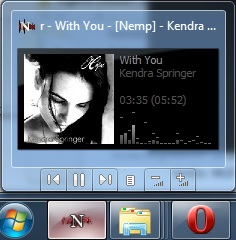
\includegraphics[scale=0.4]{taskleiste.jpg}
%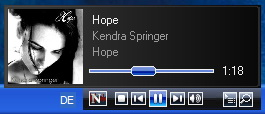
\includegraphics[scale=0.4]{deskband.jpg}
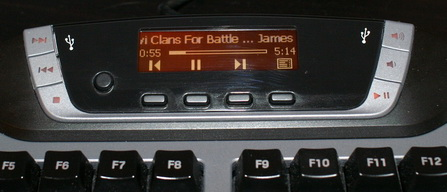
\includegraphics[scale=0.4]{g15.jpg}
\end{center}
\end{itemize}


\subsection{Skins, individual windows and form customizer}
Nemp can not only be displayed in the normal Windows look, but also uses its own appearance by default, which is also modifiable, so called \textbf{Skins}. Besides, there are two window modes, the \textbf{compact view} in which all is arranged in one window, and the \textbf{individual window view} in which the individual areas are displayed in separate windows which can be hidden and moved individually.

You can switch between the two display modes via the menu \emph{Settings - View} or via \texttt{F7}.

The individual windows dock together and can then be moved together using the player part.

\begin{figure}[tbh]
\centering
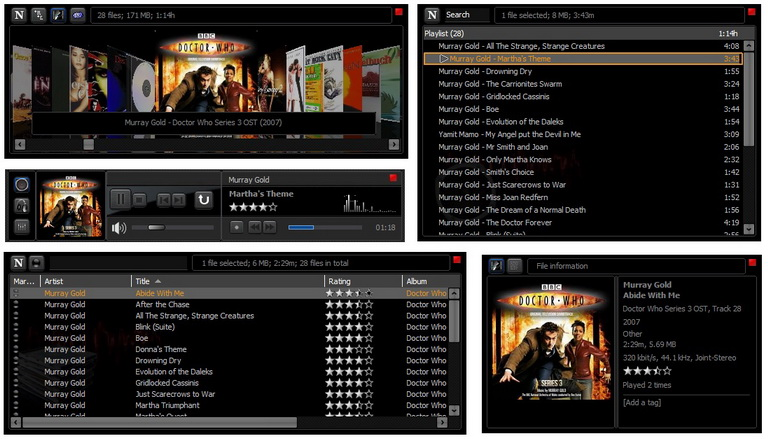
\includegraphics[width=0.8\textwidth]{einzelfenster_en.jpg}
%\caption{Unterteilungen im Hauptfenster von Nemp}
\label{fig_einzelfenster}
\end{figure}

Since version 4.11, the arrangement of the individual areas in the compact view can be configured. Thus, for example, a flat, wide \emph{coverflow} can be displayed just as well as a rather narrow, high area for browsing in the \emph{classical view}.

Of course, this has no influence on the view in single window mode - here the individual parts could always be arranged freely.

For setting the appropriate configuration there is the \textbf{Form-Designer}, accessible via the menu. The blue arrows can be used to move the individual sections. The settings on the right side should be mostly self-explanatory. 

\begin{figure}[tbh]
\centering
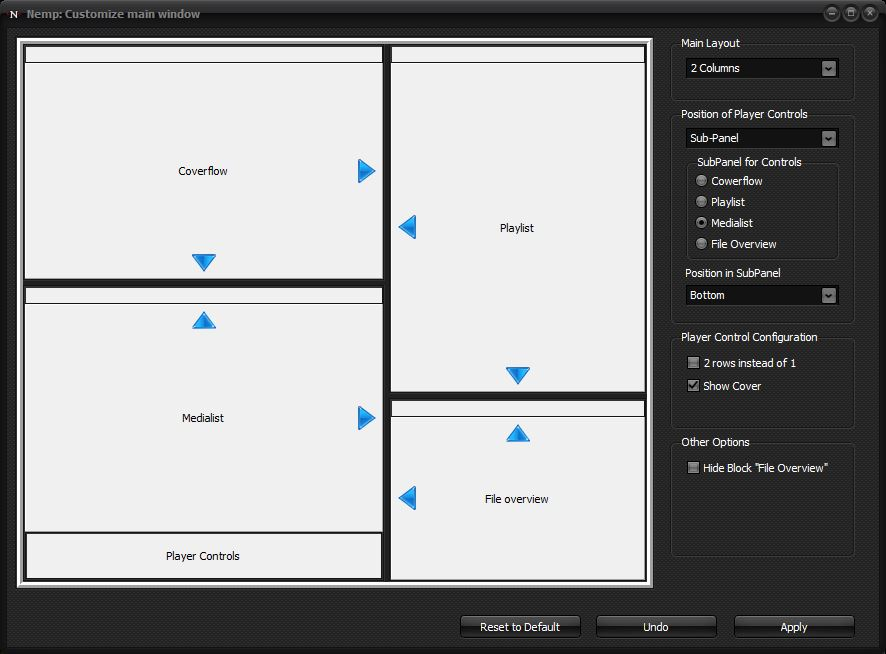
\includegraphics[width=0.6\textwidth]{form-customizer.jpg}
\label{fig_formcustomizer}
\end{figure}

\begin{itemize}
	\item The \emph{Main layout} controls whether the primary division of the window should be horizontally or vertically.
	\item Via \emph{Position of control panel} you can specify the area with the controls. This can be set to either the top or bottom, or centered in a layout with two rows. In addition, this part can be arranged with \gf{half width} at one of the other four areas - at the top or bottom.
	\item Under \emph{Control panel configuration}, the control panel can be configured a little bit. 
	\item With \emph{Other settings} the part with the file overview can be hidden, as it's not used by all users. If this part is hidden, a single-line or single-column view is also possible. If all four areas are visible, this does not make sense. 
\end{itemize}

The proportions are adjustable as usual at the dividing lines. Click on \emph{Apply} to transfer the layout to the main window, click on \emph{Undo} to return to the current layout of the main window in the Form Designer. If you have completely messed up the settings, you can restore the original layout by clicking on \emph{Reset to default}.


\subsection{Party mode}
\label{sec_partmode}

The party mode was basically a literal crazy idea. If Nemp runs on a party and takes over the sound system, then after a few (or a few more) beers the buttons become quite small and are hard to hit. In Party mode, they get bigger.

Some of the player's features are disabled in party mode to prevent accidental changes to the library or individual files. Also it is not possible to delete the complete playlist at once - you have to remove the titles one by one in party mode.

Party mode can be secured by a password, which has only an alibi function. It does not prevent that Nemp can be terminated and then restarted in normal mode.

\subsection{Languages}

Nemp is basically designed to support multiple languages. The original language is English for compatibility reasons. 

Due to a lack of language skills, I cannot offer any other languages besides english and german myself. However, the system is designed so that theoretically everyone can produce a further translation. If you are interested, you can download the so-called Po-Editor from \texttt{https://poedit.net} for a first look, and decompile the file \texttt{default. mo} in the folder \emph{Languages{Languages}} (or the other subfolders) in the Nemp folder (via the Windows Explorer context menu), and then open the file \texttt{default.po}  with the Po-editor. In principle, you can then start right away and translate everything. Some translations must follow certain rules. For example, the number and sequence of certain strings such as \texttt{\%s} and \texttt{\%d} must remain the same, as they are filled by Nemp with matching pieces of text or numeric values.

For more information please send me an e-mail and we'll see. But as a warning: This is a sh*** job. ; -)


\subsection{External drives and backups, portability}

One of the main goals in developing Nemp was portability. Nemp should not need to be \emph{installed}, but should simply run like this - including the media library. Even if Nemp resides on an external hard drive with the entire music collection, and when connecting the drive, all the data is stored sometimes on \verb+D:\+ and sometimes on \verb+E:\+.

For this purpose, the media library stores not only the paths to the individual music files, but also information about the drives on which the data resides. Nemp examines the drives at start and corrects the path information if necessary. 

This also works while Nemp is running. For example, if you forgot to connect the external hard drive with your music collection before starting Nemp, it doesn't matter. As soon as it is connected, Nemp notices this and automatically adjusts the paths.

This method works very well in most cases, but has one gap: If you have your complete collection on two different drives, i. e. an original and a backup, then Nemp will differentiate between these two drives, even if both always appear under the same drive letter in the system. Because of the automatic drive adaption it will not find the files then when you connect the other drive - even though the files are there. Nemp \emph{does not} corrects the paths in that case, but makes them \emph{kaputt}. The workaround is to always connect the same disk, or to make two copies of the media library and load the appropriate media library, depending on the hard disk.




\section{Player and Playlist}

In the following we will take a closer look at the actual player and the playlist, which cannot be separated from each other.


\subsection{Display and controls in the player}
\label{sec_anzeige}

In version 4.11, the control of the player has moved to another position. Formerly centered in the upper part of the window, it is now at the bottom. The layout and accessibility of some functions has also changed.

Nemp's control panel is divided into four parts.

\begin{figure}[tbh]
\centering

\includegraphics[width=0.6\textwidth]{player.jpg}
\end{figure}


\begin{itemize}
\item At the left is a small area to choose from. Here you can switch between the control of the main playback and the headphone output (useful for a second sound card). Since Nemp 4.11 the equalizer and the effects are controlled in a separate window.
\item Next to it is a small picture with the cover of the current title. This area can be hidden in the Form Designer.
\item In the middle the control of the player. Play/Pause, Stop, Next/Previous Track, Playback mode and Volume.
\item The broad section shows some information about the current title - artist, title, rating and progress indicator. There are also buttons for recording (webradio only) and for jumping back and forth within the current title (files only). 
\end{itemize}


For the playback mode, the individual symbols mean:

%\begin{center}
%
\includegraphics{BtnRandom.png}
%\end{center}
\begin{itemize}
 \item[] \inlinegraphics{BtnRandom1.png} Repeat all: Nemp runs through the playlist from top to bottom and then starts again. 
 
 \item[] \inlinegraphics{BtnRandom2.png} Repeat title: Only the current title is repeated. 
 
 \item[] \inlinegraphics{BtnRandom3.png} Random mode: The files are played back in random order. In the options you can set whether the \emph{true randomness} should be modified to achieve a \emph{seemingly more random} behavior, or to select the titles depending on your rating with higher or lower probability. For more information on random play, refer to the section \hyperref[sec_random]{random playback}. 
 
\item[] \inlinegraphics{BtnRandom4.png}  Do not repeat: Nemp plays the playlist and then stops playback. 
\end{itemize}

In the middle part the active \textbf{Tools} are listed additionally by small icons (not visible in the picture above). For details see chapter \hyperref[sec_tools]{Tools}.

\begin{itemize}
\item[] \inlinegraphics{shutdown.png} The shutdown countdown has been activated. You can find out exactly what happens when (e.g. shutdown or hibernation) with the hint text on this icon. 
\item[] \inlinegraphics{geburtstag.png} The birthday mode has been activated. Nemp will automatically interrupt the playlist playback for a birthday song in due course. 
\item[] \inlinegraphics{webserver.png} The web server is enabled to allow access to the player via a web browser. 
\item[] \inlinegraphics{scrobbler.png} Scrobbling is activated. The songs you are listening to at the moment will be transferred to your user profile on last.fm.
\item[] \inlinegraphics{warning.png} Low battery - Playback is littering. A small fun feature for laptops that only run on rechargeable batteries. The Walkman mode is active and the battery is low. Nemp will then begin to litter to let you know that you should plug the laptop into the power supply.
\end{itemize}

\subsubsection{Equalizer and effects}

With the \textbf{Equalizer} you can adjust the playback. But that's not much more than a gimmick, audiophile users probably won't have much fun with it.

\begin{center}
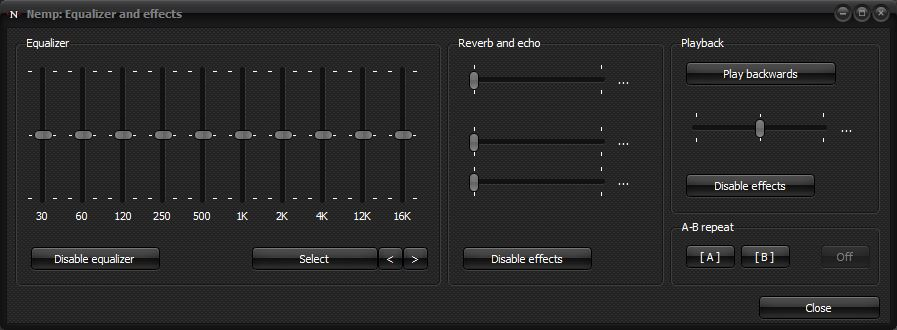
\includegraphics[width=0.6\textwidth]{eq.jpg} 
\end{center}

The same applies to the \textbf{effects}. A little bit of reverb and echo can be added and the playback speed can be increased or decreased. Since Nemp 4.12 the \emph{Micky-Mouse-Effect} can be switched on and off directly. Also, since version 4.12 there's the \gf{Wobble playback} effect, which was previously only implemented as a hidden feature as a warning for low battery.

\begin{tipp}
Right-clicking on a controller brings it back to the 0-position.
\end{tipp}

Another gimmick is the \textbf{reverse playback} of the current title, and the \textbf{A-B-repeat}, which repeats a certain section of the current title in a loop. Clicking on A sets the start point, clicking on B sets the end point, and pressing X deletes both so that the playback continues normally.

\begin{tipp}
If you have set the start point A and end point B, you can also move the knobs in the control panel of the main window.
\end{tipp}


\subsubsection{Headphones}
\label{sec_headphones}

A special function in Nemp is the built-in \textbf{headphone playback}. This can be placed on a second sound card (this can also be done with a small USB sound card for a few euros/dollars) to listen to a song without disturbing the actual playback.

\begin{center}
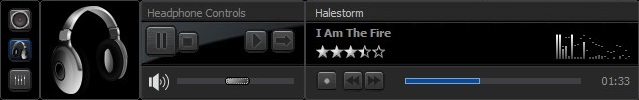
\includegraphics[width=0.6\textwidth]{head.jpg} 
\end{center}

With Nemp 4.11, the headphone playback control changes a little - it now shares the space with the actual playback control. Switching is done with the buttons on the left side of the control panel.

To insert a title into the headphone playback, you can use the key combination \texttt{Ctrl+H}, or you can drag and drop a title into it.

Additional controls there are

\begin{itemize}
 
 \item[] \inlinegraphics{BtnHeadsetToPlaylist.png}  Inserts the current track in the headphone player into the playlist. How exactly - e.g. behind the current title or at the end of the playlist - can be defined in the settings. Or you can select the proper method from the dropdown menu of this buton.
 
 \item[] \inlinegraphics{BtnHeadsetPlaynow.png}  Inserts the current track in the headphone player into the playlist behind the current track in the playlist and immediately starts playback at the current position.

\begin{tipp} Use this function if, for example, a title has an unnecessary intro and you don't want to have long breaks at a party. 
\end{tipp}
\end{itemize}



\subsection{The playlist}

The core of each player is the playlist, i. e. the list of songs to be played.

\textbf{Enqueue files} into the playlist via the menu, by dragging and dropping them from the Windows Explorer, or by using Copy\&Paste.

You can also play many of the usual \textbf{web radio stations} with Nemp. If the sender offers a .pls file, you can simply open it with Nemp. Some other formats are also supported. You can organize your favorite stations under \emph{Media Library - Web Radio} (keyboard shortcut \texttt{Ctrl+W}).

The order in which the playlist is played back can be changed by pressing the button for the playback mode. You can also sort the playlist using the menu or drag and drop individual titles.

\begin{center}
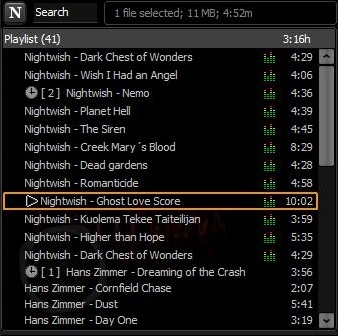
\includegraphics[width=0.4\textwidth]{playlist.jpg} 
\end{center}

New in Nemp 4.7 is the \textbf{search in the playlist}. This works similar to the quick search in the media library - just focus the search box (also works with the key combination \texttt{Ctrl+F}, if the playlist has the focus) and start typing. The first hit is selected in the playlist. Pressing the \texttt{F3} key will highlight the next hit. With \texttt{Enter} all search hits are marked, and can be copied to the clipboard via Copy\texttt{Strg+C} or \texttt{Strg+Shift+C}. With \texttt{Shift+Enter} the currently selected title is played.

Since version 4.13, Nemp ReplayGain supports ReplayGain for automatic adjustment of the Loudness. Titles with ReplayGain information are indicated in the playlist by a sound level symbol. When the automatic loudness adjustment is disabled in the settings, this icon is displayed in grayscale. More
about this in the next section.

A hidden feature is the prebook-list. You can use the \texttt{0...9} numeric keys to set a temporary individual sequence. Simply highlight the song you want to hear next and press the \texttt{1} button. Mark another one with \texttt{2} and so on. If you want to change the order, this works as well. If you want to remove a marker, press \texttt{0}.

\subsection{ReplayGain - automatic loudness adjustment}
\label{sec_ReplayGain}

Since version 4.13 Nemp supports ReplayGain. This adjusts the volume of tracks from different sources so that all tracks are played at the same volume. At least that's the goal.

Nemp evaluates the ReplayGain information in the metadata. The most common tags are in the format \texttt{REPLAYGAIN\_TRACK\_GAIN}. There are a few other formats for them, but to my knowledge they are only used sporadically and are therefore not supported by Nemp (so far). 

These tags are supported by MP3, Ogg-Vorbis, Flac, M4A and the more exotic formats that use the APEv2 tag for metadata. These values must be calculated in advance, which takes some time. 

\subsubsection{The concept behind ReplayGain}

\textbf{TrackGain.} ReplayGain tries to make all titles sound equally loud. The volume of a title is compared with a reference value. The deviation from this reference value indicates to what extent the volume of the title must be increased or decreased during playback so that this reference value is reached. This value is called \emph{TrackGain}.

\textbf{AlbumGain.} Some albums, however, have titles that are intentionally louder or quieter than other titles on the album. These intentional differences in volume would then be lost. Therefore, not only the volume of the individual tracks is analyzed, but also the average volume of the entire album is considered and the difference to the reference value is determined. This is the \emph{AlbumGain} value.

Depending on the playlist, either TrackGain or AlbumGain should be used. This can be set in the settings dialog under \emph{Player Settings}.

\textbf{Pre-amplification.} Depending on the music collection, it makes sense to define a default value for the volume adjustment. Many current albums are mixed very loudly (keyword \emph{Loudness-War}). Thus the ReplayGain values for these tracks are negative (e.g. -6dB). If a title is played without ReplayGain information, it may appear disturbingly loud. A default value of e.g. -5dB significantly reduces this difference. 

On the other hand, after using ReplayGain in this example, all titles appear (significantly) quieter than before, which is also not always desired. Therefore an additional default value for title \emph{with} ReplayGain data can be specified.

These default values disable ReplayGain a bit. Which values make sense depends on your own preferences and on the composition of the music collection.

\textbf{Clipping and Peaks.} If a positive value is set for the preamplification, then it can happen that some samples are amplified beyond the actual maximum. This results in disturbing effects during playback, called \emph{clipping}. To avoid this, the volume increase can be adjusted so that the peak value of a title is never amplified beyond the maximum. Therefore, when calculating the ReplayGain values, the peak values are also calculated and written into the metadata (as \texttt{REPLAYGAIN\_TRACK\_PEAK}, correspondingly also for the album value.

These options can also be changed in the \emph{Player Settings}.

\textbf{Clipping and Floating-Point-Channels.} By default, Nemp uses floating point channels for playback. These channels also allow internal processing of samples beyond the \gf{actual maximum}. A possible \emph{clipping} only occurs at the speakers - if at all. Therefore, the \emph{Prevent Clipping} option does not improve the sound in many cases, but only reduces the volume. However, if you disable the use of floating point channels in the \emph{Advanced Player Settings}, and then set high values for preamplification, you'll hear the effect of \gf{Prevent Clipping} very clearly.

\subsubsection{Calculation of the ReplayGain values}

With Nemp these values can also be calculated, if they are not already available. First select some titles in the playlist or media list and then select the item ReplayGain or the desired variant via the context menu (right click).
\begin{itemize}
\item \textbf{individual titles.} Only TrackGain values are calculated. 
\item \textbf{as one album.} In addition to calculating the TrackGain values, the selected tracks are taken as one album. The AlbumGain values are based on the average volume of all selected tracks. 

In order to minimize the number of write accesses to the metadata, the TrackGain values are only written to the metadata when the AlbumGain values are available - i.e. after the last title has been calculated. If the process is aborted before the end, all calculated values will be lost.

\item \textbf{multiple albums (by tags).} The selected files are interpreted as multiple albums. The automatic compilation of the albums is based on the metadata. If the value for \gf{Album} in the metatags differs (e.g. because the appendix \gf{CD 1/2} is contained), this option should not be selected. 

The ReplayGain values for an album will be written to the metadata when the calculation of all tracks for that album is complete.
\item \textbf{ReplayGain values delete.} The values will be deleted from the metadata again.
\end{itemize}

A few hints about that:
\begin{itemize}

\item The audio data itself is not changed. Only up to four data points (track/album gain/peak) are inserted into the metadata of the files. Players that do not support ReplayGain are not affected. Players that support ReplayGain in this form, of course are. 

There is also the variant (at least with mp3 files, see \emph{MP3Gain}) that the audio data itself is changed (reversibly), so that even with players without ReplayGain support there is an even volume. This method is \emph{not} used by Nemp.

\item It is absolutely not recommended to calculate the ReplayGain values for the entire media library at once. This is especially true for the \emph{multiple albums} option, because even with well-maintained collections, the album subdivision is not always 100\% correct.
And of course this applies even more to the \emph{as one album} option - applying it to the entire media library (or to large parts of it) is absolutely pointless. Because this way (when using the AlbumGain values) the differences in volume are preserved, which ReplayGain is supposed to prevent.

\item To calculate the AlbumGain value, all titles of the album must have the same sample rate. For example, if one title does not have the usual 44.1kHz, but 48kHz, then the calculation of the AlbumGain value is aborted.

\item During my tests it turned out that Nemp (or the used program library) delivers slightly different values for some files than e.g. foobar2000 or Mp3Gain. The deviations become particularly clear with titles that have both very loud and very quiet passages. However, the tendency is correct, and for titles with strongly fluctuating volume (as a classic I refer to the \textit{Bolero}) an \gf{average} Volume anyway is a term difficult to define, resp. is such a value there only of very limited expressiveness.


\end{itemize}













\subsection{Special features}

Over time, a few (more or less) useful functions and functionalities have been added.

\begin{itemize}
\item If a title is selected in the media library, then it can be played as \textbf{Jingle} additionally. Press \texttt{F9} and hold down the button. Nemp plays this song in parallel to the main playback while the F9 key remains pressed. 

\item The key \texttt{F8} serves as a \textbf{Push to Talk}. This will decrease the volume as long as the F8 key is held down. 

\item With \textbf{Enhanced Copy\&Paste} via \texttt{Ctrl+Shift+C}, the marked files are copied to the clipboard (as with the known \texttt{Ctrl+C}). In addition, a suitable playlist file is created and inserted into the clipboard. 

The purpose of this additional playlist file is to allow the selected titles, which may have confused filenames, to be inserted into a playlist in the same order in which they are currently sorted in the playlist.

\item If that's not enough, there is the menu item \textbf{Copy Playlist}. This will copy the titles in the playlist to a new directory with (if desired) new filenames.

\item If an audio file (e.g. mix CDs) has a *.cue-file of the same name (so-called \textbf{Cue-Sheets}), then this file is evaluated, and the individual titles of the mix can be accessed directly. 

\item Via the menu you can create a \textbf{random playlist} from your music collection according to certain criteria. 
\end{itemize}


\section{The Media Library}

Nemp can search for audio files on your computer, manage them in a media library, and view them sorted by criteria. Using a quick search, you can find the desired title in no time at all and add it to the playlist.

\emph{That was the first thing Nemp could do. Nemp was originally not a stand-alone player, but only an MP3 manager with a connection to Winamp. Only after the first presentation in a developer forum did the suggestion to make it a player came up... }


\subsection{Building the Media Library}

To add new files to your media library, choose \emph{Media Library - Scan hard disk for audio files} from the menu and select the folder containing your music files. Nemp then scans this directory, including all subfolders, and inserts the audio files found into the media library.

This process can take some time - Nemp can handle about 20-40 files per second. You can continue to use Nemp during this time - even if some things don't run as smoothly.

Alternatively, you can simply drag your music folder to the Media Library area. So into the upper left area, or the entire lower area. Just don't put it in the playlist.

\subsection{Browsing the Media Library}

There are three basic ways to browse the Media Library. You can switch between the three browser modes with the buttons in the upper area. The \textbf{classic view}, the \textbf{coverflow} and the \textbf{tag cloud}.

\begin{center}

\includegraphics{TabBtnBrowse.png}
\end{center}


\subsubsection{Classic view}

The classical view was there first. The media library is displayed here filtered according to two criteria - e.g. artist and album. In the left half all artists are listed. If you select an artist, the list displays all albums and samplers where this artist is represented next to it, and the large list below shows all the songs of this artist.

Via the context menu \emph{Browse by -... } you can select the criteria according to which you want to browse in this view.


\subsubsection{Coverflow}
\label{sec_coverflow}

The coverflow sorts the songs by covers. For this purpose, Nemp not only scans the music files when searching for audio files, but also searches for a suitable cover for each song in the ID3 tag of the file or on the hard disk. 

For this purpose, Nemp assumes that the folder structure is roughly the same as the album structure, i.e. you have one folder on your disk per album. For the definition of an \emph{album}, Nemp primarily takes the folder structure.

If no cover is found, Nemp can search the internet for a suitable cover.


\begin{center}
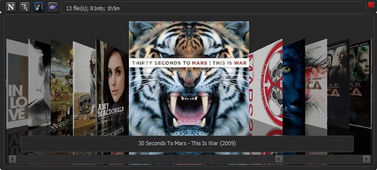
\includegraphics{browse_coverflow.jpg}
\end{center}

In detail, this works as follows. First, each mp3 file is scanned for a cover in the ID3 tag. If there is one, that is taken. 

If there is no cover in the ID3 tag, image files are searched for on the hard disk \emph{near the audio file}. From this picture list, the picture that looks like a \emph{front-cover} is taken. I.e. a file is searched for which has an \texttt{front}, a \texttt{\_a} or a \texttt{folder} in the name (with this priority).

All files to which the same cover was found with this method are grouped under this cover and interpreted as an \emph{album}.

Files for which no cover can be found are grouped by folder. 

What exactly means \emph{nearby}, can be specified in the \hyperref[sec_coversettings]{\emph{search}} settings. 

You can sort the \textbf{Coverflow} by selecting \emph{Browse by -... } as in the classic view from the menu. Note that the artist or album name of the whole album is taken - for a sampler the artist is often \emph{Various Artists}.

If no cover is found for a song, Nemp can search the Internet for a matching cover. Nemp uses the last.fm API, which is also used for scrobbling. However, no registration is required for the cover search. It just works like this.

\begin{tipp}
Use the \hyperref[sec_wizard]{\emph{Nemp Wizard}} to allow searching for covers on the Internet. 
\end{tipp}

If a new cover has just been downloaded from the Internet, Nemp displays a small icon on the cover.

\begin{itemize}

\item[] \inlinegraphics{lastfmOK.png} The cover has just been successfully downloaded and saved by last.fm. A copy of it can now be found in the folder of the audio files named \texttt{front\_(NempAutoCover).jpg}. 

\item[] \inlinegraphics{lastfmFail.png} No cover could be found on last.fm either. This happens with exotic albums and (unfortunately) very often also with samplers. 

\item[] \inlinegraphics{lastfmCache.png} 
The request to last.fm was not executed, because another attempt failed recently. There will be a daily (or later only weekly) request until the cover search for this album will be stopped completely. You can delete this \emph{cache} with already unsuccessfully retrieved covers in the settings dialog.

\item[] \inlinegraphics{lastfmConnectError.png} No connection to last.fm could be established. Usually this is due to a missing internet connection or the settings of your firewall. If you receive this ad with all new covers, please contact me. It may well be that something has changed in the web service and a Nemp update is necessary.

\item[] \inlinegraphics{lastfmInvalid.png} This icon does not appear in the coverflow, but only in the cover view of the player. It indicates that no uniform album information can be found for the files in the same folder as the current track. In this case, the search at last.fm is skipped. 
\end{itemize}

\subsubsection{Tag cloud}
\label{sec_tagwolke}
In the tag cloud, all properties such as artist, album, genre, year, year, decade are thrown into one big pot and the most common properties are displayed - always as much as there is room in the window. If you click on such a \emph{tag}, you will get all titles with this tag displayed. If you double-click a tag, a new tag cloud is created, which only takes titles with that tag into account.

\begin{center}
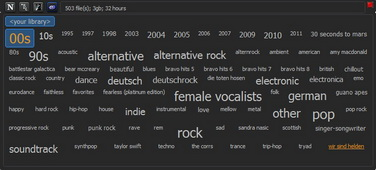
\includegraphics{browse_tagwolke.jpg}
\end{center}

For the tag cloud, the properties artist, album name, genre, year and decade (e. g. \emph{90s}) of the titles are initially thrown into one pot in the media library. The most frequent of these \emph{tags} are then displayed in a cloud, as one knows them from many web pages.

You can then, for example, select the tag \emph{00s} or \emph{90s} and get all titles from the 2000s or 90s displayed. If you double-click on this tag (or press the Enter key), a new tag cloud is created from these titles - you can continue to do so almost at will.

The interesting thing is now the possibility to assign additional tags to the titles, which are also stored in the mp3 files themselves. For example, you can assign several genres to a title. Or enter other comments that classify the song.

Of course, it's a bit of a hassle to do this for every single song in the entire media library. But what is the Internet for? At last.fm there are not only covers, but also other tags maintained by the community - maybe you've already tagged a few songs about it yourself.

Nemp can query the most common tags for a song at last.fm and store them in the media library. To do this, select the files you want to tag and choose \emph{Get additional tags from last.fm} from the menu.

\begin{hinweis}
This only works if the files already have proper standard ID3 tags like artist and title. And it'll take a while. Firstly, the Internet is slow, and secondly, the admins at last.fm become nasty when a program overloads the API. About 2-3 files per second are ok, that's all. Nemp therefore deliberately slows down the enquiries.
\end{hinweis}

With these additional tags, the tag cloud becomes a little more meaningful. Unfortunately, last.fm has a lot of tags in different spellings, which causes a little bit of clutter. A workaround for this is provided by the built-in tool \hyperref[sec_tagwolkeneditor]{tag cloud editor}.

\subsubsection{Browsing via the display}
\label{sec_titleinformation}
Regardless of the selected mode (classic view, coverflow, tag cloud) you can browse through the currently highlighted titles in the media library. 
\begin{center}
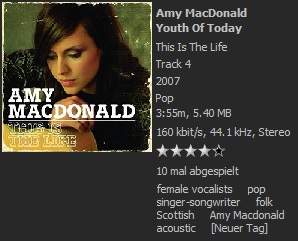
\includegraphics[width=0.6\textwidth]{tags.jpg}
\end{center}

A double-click on the artist will list all songs of this artist, a double-click on the album will list all songs of the album, etc. etc. Only exact matches are listed. A double-click on the title \emph{Angels} from \emph{Robbie Williams} will not cause any titles of \emph{No Angels} to be listed, nor will other titles such as \emph{When Angels cry} from \emph{Beyond the Black}. This also applies to the extended tags. Even if an extended tag is set here that corresponds to the artist or year of publication. Nemp has no built in logic which can tell, whether an automatic tag could be interpreted as \emph{interpret}, \emph{genre} or \emph{year}. Double-clicking on an extended tag will only list the files in which this \emph{extended tag} is explicitly set.


\subsection{The quick search}

If you want to listen to a certain song, you can use the quick search function. Focus the search box (you can also use the key combination \texttt{Ctrl+F} as long as you are not in the playlist (this will take you to the playlist search) and just start typing. Nemp will show you all the titles that match the current search term while typing. 

With \emph{*} you can search for all titles in the media library. If you really want to see all titles containing a \emph{*}, you must escape the asterisk with \emph{\textbackslash*}.

Since Nemp 4.9.2 the last 10 search terms are logged and can be retrieved via the context menu of the quick search input field.

\begin{tipp}
By default, \emph{during typing} only exact hits are listed. When you press the \texttt{Enter} key, Nemp performs an fuzzy search that also takes spelling mistakes into account. Then titles of \emph{P!nk} will also be found if you searched for \emph{Pink}. And if you are not sure how many \emph{r}, \emph{s} and \emph{t} occur in \emph{Alanis Morissette}, that's not bad either.
\end{tipp}

\subsection{Set markers and use them}

With Nemp 4.8 the possibility to mark files with \emph{markers} was added. These markers can be used to highlight some of your music files. They can be set via the context menu, the key combination \texttt{Ctrl+Shift+1} (or \texttt{+2, +3}, to remove \texttt{+u}), or by clicking on the column \emph{mark}. By default, this column is not visible - use the settings dialog to display it or use the context menu of the column headers. Currently, three different markings are possible.

\begin{center}
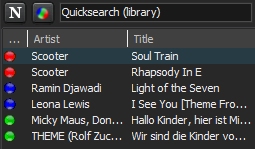
\includegraphics{marker-en.png}
\end{center}

To view all marked files, click on the button next to the quicksearch. Then all files are displayed with the respective marker. Repeated clicking will switch the displayed marker accordingly.

In the display settings you can set whether files marked accordingly from the entire media library or only those from the current preselection are displayed.

The coverflow, search, quicksearch and other ways to search and browse the library will ignore these markers.

The markers are stored only in the Media Library and not in the ID3-Tag of the music files.

\subsection{The detailed search}

In most cases, the quick search is sufficient. Only in a few cases, e.g. when searching for a certain song text, the detailed search must be used. This was one of the first functions in the prototype Nemp, which was actually just an mp3 management tool. You can access the search via the menu or the key combination \texttt{Ctrl+Shift+F}. In the search window, enter the search terms and search for them.

By default, the fuzzy search is activated, which also lists search hits with small deviations. This can also be deactivated. The number of errors in the fuzzy search is defined by the so-called Levenshtein distance. Depending on the length of the search term, more or less errors are allowed. An error is the insertion, deletion or modification of a character.

So don't worry about the exact spelling or typos - especially when searching for lyrics. Also a search for \emph{in the taun wer i was born} leads to the desired title \emph{Yellow Submarine} with the line \emph{in the town, where i was born}.

%With \textbf{Search} a new search is started. With \textbf{Refine search} is searched only in current search hits, and with \textbf{Extend search} new ones are added to current search hits.

Restriction to \textbf{genre} or \textbf{year} is still in it for nostalgic reasons, but in most cases probably more obstructive than useful.

As a bonus, the last search history is saved and can be called up again.

\subsection{From the Media Library to the Playlist}

You can insert a single track, or a few tracks, or an entire album, or all songs with a specific tag, or anything else into the playlist - either from the context menu or by dragging and dropping. You can also start Drag\&Drop from the coverflow or the tag cloud.

Drag\&Drop and Copy\&Paste have a limit of 2500 files. This is a protection against operating errors with the player crashing afterwards - with too many files in the clipboard, Windows will have problems at some point. The context menu is always available for inserting any number of tracks into the playlist.

If you double-click a single title in the lower list, then what you have set as the default action in the settings dialog happens.

\begin{itemize}
\item \textbf{Enqueue at the end of the playlist} (default). The title is appended to the end of the playlist 
\item \textbf{Play (and clear current playlist)}. The current playlist is emptied and a new one is started eith the selected track.
\item \textbf{Enqueue after current track}. The new title is inserted after the title that is currently being played.
\item \textbf{just play}. Playback of the playlist is interrupted and the song is played \emph{simply so}. If you click on \emph{next title} in the player, playback of the playlist restarts at the interrupted position. 
\end{itemize}

\begin{tipp}
Drag\&Drop also works from Nemp to other programs, e.g. to copy a song to a mobile mp3 player. 
\end{tipp}

\subsection{Maintenance of the Media Library}

For proper sorting and quick retrieval of the files, it is important that each audio file has proper metadata.

Nemp 4.6 supports the following systems:

\begin{itemize}
\item ID3-Tags (version 1, 1.1, 2.2, 2.3 and 2.4) 
\item Ogg-Vorbis-Comments
\item Flac-Metadata 
\item Apev2-Tags 
\item iTunes Tags 
\end{itemize}
Thus, Nemp supports metatags in *.mp3, *.ogg, *.flac, *.ape, *.mpc, *.ofr, *.tta, *.wv and * m4a. Not fully supported are *.wma (Windows Media Audio) - tags can be read from these files, but writing is not supported.

\subsubsection{Simple editing of metadata}

Nemp doesn't include a tag editor to set tons of ID3 tags, but editing individual ID3 tags works fine with it. Simple properties such as title and artist can be edited directly in the list. Simply select a title, navigate to the corresponding column and click slowly twice, or press the \texttt{F2} key.

You can edit the extended tags in the additional display to the right of the list. To change or delete an existing tag, you can use the context menu (pointing to the tag with the mouse, right-clicking, selecting the desired action). For a new tag, either use the context menu or double-click on \emph{New tag}. You can also enter several tags separated by commas at the same time. 

If the basic information artist and title in the files are set appropriately, Nemp can automatically retrieve song lyrics and extended tags from the Internet. Lyrics are useful if you can't remember the title, but only one line of the song. Extended tags are needed for better browsing in the \emph{tag cloud} mode.

\begin{hinweis} This direct editing of meta-information is only possible if quick access to meta-information is allowed. This can be done via the \hyperref[sec_wizard]{Nemp Wizard}, or in the settings dialog under Metadata. 

This does not apply to the rating of titles. This is always possible. However, if the metadata in the settings has been disabled, the ratings entered are saved only in the library, not in the files themselves. This means that the ratings are not available in other players, and that they may get lost when the media library is rebuilt.
\end{hinweis}


\subsubsection{Updating the data}
If you have changed individual files with other programs, you can reload these files. To do this, select \emph{Refresh selected files} or \emph{Media Library - Refresh} from the context menu. For a few files this is still quite fast, but the complete re-reading of a media library with some 10,000 titles takes a few minutes.


\subsubsection{Deleting files and cleaning up the library}

To delete files from the Media Library, select \emph{Remove selected files}. This deletes the files from the library, but not from the hard disk. 

If you have moved parts of your music collection to other folders, the file paths in the Nemp Media Library are invalid. You should then remove non-existing files (\emph{Media Library - clean up}) and, if necessary, add your (new) music folder to the media library.

\subsubsection{Webradio}

Nemp can not only manage files, but also a list of web radio stations you listen to regularly. But: Nemp is primarily an mp3 player, not a radio. The function is included, but the focus is not on it.

In the classical view in addition to files also \textbf{webradio favorites} are displayed. You can edit this list using the menu \emph{Media Library - Manage Web Radio Channels} and insert new stations.

You can choose the name of the sender freely, as URL you should enter the address of the sender. Very often one gets these on the respective web page - on most cases there is a link which ends on \texttt{.pls}. You must enter this link in the URL field. Many channels or websites offer different links for the Windows Media Player, Winamp or maybe even the Real Player. Nemp should be able to handle the Winamp link.

You can also sort the favorites list according to your wishes.

\subsubsection{CSV export}

A special feature is the possibility to export the complete media library as a csv-file, including most of the data. Excluded are lyrics (it is only exported if there are any) and extended tags. This csv file can then be imported by many other programs (e.g. Excel).

\subsection{The detail window for editing metadata}
\label{sec_details}

For a more detailed editing of meta information, Nemp has a \textbf{detail window} that can be opened with the key combination \texttt{Ctrl+D} when a title is highlighted in the media library or playlist. In addition to specific changes to the ID3 tags, other information can also be retrieved here which is not necessarily of great interest, but which some might find useful.

This window has been completely redesigned for version 4.13.

\begin{hinweis} If you make changes in this window and click \emph{Apply}, the entries are always saved in the file's metadata. Even if the quick access to the metadata is not allowed in the settings.
\end{hinweis}

Some inputs on the different sides of this window may contradict each other. For example, if you change the title on the first page (\emph{summary}) and also change the frame for \gf{title} on the \emph{metadata} page, inconsistencies or unexpected behavior may occur when saving to the file. Therefore, Nemp will warn you when you change the page if any changes have been made that have not yet been saved.

\begin{figure}[bth]
\centering
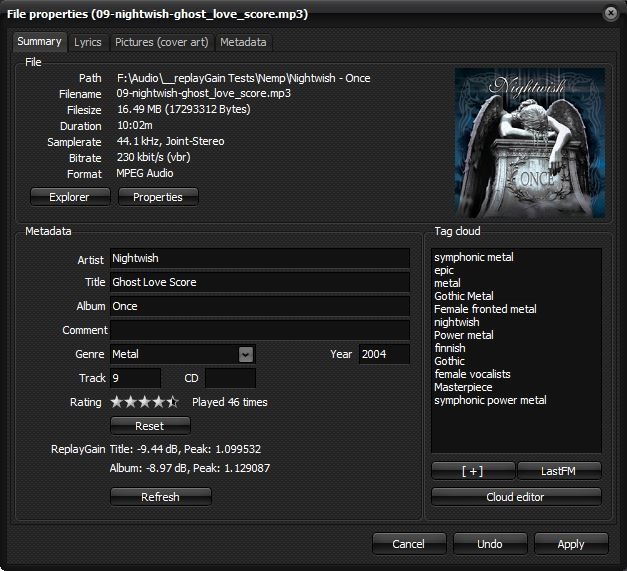
\includegraphics[width=0.9\textwidth]{details_a.jpg}
\label{fig_detailfenster}
\end{figure}

\subsubsection{Summary}

The first tab \textbf{Summary} gives you an overview of the meta data for the selected title. The button \emph{Explorer} opens the Windows Explorer with the folder of the file, via \emph{Properties} you get the Windows properties dialog.

Since Nemp 4.13 it is possible to edit the basic values like title and artist. Rating and playback counter are not editable directly, but can be set back to 0 by a button click (\gf{0} for the rating are 3.5 stars). The ReplayGain values are also only displayed there. The extended tags for the tag cloud can be edited.

\subsubsection{Lyrics}

The second tab is intended for displaying and editing lyrics. The lyrics can be edited freely, or can be obtained automatically from currently two sources on the net.

If you want to edit lyrics for multiple titles, it might be faster to use the multiple search for lyrics. To do this, select several files in the main window and select the \emph{Get  Lyrics} function (key combination \texttt{Ctrl+L}). This will take a little time, and not all titles will be found with the correct lyrics, but the hit rate is quite good.

Since version 4.10 not only the page \emph{lyrics.wikia.com} is used, but optionally also \emph{chartlyrics.com}. Which source is used with which priority can be set in the options. The new page Chartlyrics should only be used as fallback. When searching on this page, some search terms will be filtered out automatically. For example \emph{are, take, that, the, who, are, you} and many others. What effects this will have on the titles from Bands like \emph{Take That} or \emph{The Who} (especially the title \emph{Who are you?}) you can then imagine yourself.


\subsubsection{Pictures (cover art)}

The third page is reserved for Cover-Art, and with 4.13 there is an extension of the functionality, which I wanted to add for a long time.

Here are listed all pictures Nemp found for the title. Both in the metadata (several pictures can be stored there) and as a file on the hard disk. Both (often hidden) system files like \emph{folder.jpg} and explicit cover art files like \emph{(my-album)-front.jpg} are found. The available images can be displayed via the selection boxes.

A new role is assigned to the display of the image that Nemp currently uses for the main window and coverflow. New is that this image can be \emph{changed} without tricks. This is useful, for example, if Nemp's heuristic for searching the \gf{Front-Cover} returns an unwanted result, or if Nemp tears an album apart because of individual image data in the ID3 tags in the coverflow \gf{...}. 
\begin{itemize}
\item The button \emph{Load cover art} can be used to select any image file as a cover for the media library. 
\item Click on \gf{Use current selection} to use the image currently selected from the list of automatically found images (metadata and files). 
\item \emph{Reset} deletes a previously manually set cover, and Nemp selects one on itself again.
\end{itemize}

Click on \emph{Apply} (at the bottom) to save the newly selected cover. If the \emph{Update all files with this cover} checkbox is checked, the new cover will be set for all files that previously used the old cover art.

After that the coverflow may have to be updated. This does not happen automatically, but only after clicking on the button, which is then displayed at the bottom.


\begin{hinweis} This selection of the album cover remains even if the media library is updated and the metadata is re-read. Nemp writes an ID calculated from the selected image into the metadata of the audio files. If this ID is present in the metadata, this cover will be used for display if the corresponding file is present in the cover folder.
\end{hinweis}

\subsubsection{Metadata}

On this page you can find further information from the metadata. For MP3 files, the older and more restricted ID3v1 tag is also displayed here. Otherwise \gf{only} the listing of (almost) all existing metadata in the file. Some of these can be edited, others not (grey font). Some of the values not editable on this page can be edited in other ways, e.g. lyrics or covers.

Data fields that do not only contain plain text are displayed as far as possible up to a certain length (non-printable characters as dots). Larger amounts of data are only displayed as \emph{Binary Data}, followed by the size of the data.

To edit, double-click an entry or press the \texttt{F2} key. With the button \emph{New Frame} further text information can be inserted. Which information is possible depends on the format of the audio file. Even if some formats like Ogg or Flac allow any tags in principle, Nemp offers only a selection here.

\begin{hinweis}
The access to the metadata is done here on a quite elementary level. If you are not sure what e.g. \gf{new frame} means in this context, or what the possible frames mean, then leave that alone. However, nothing should break the files, and other players should not have any problems with any of the data entered here - in the worst case they will simply be ignored.
\end{hinweis}


\subsection{The tag cloud editor}
\label{sec_tagwolkeneditor}

The automatic retrieval of additional tags for the tag cloud via last.fm is a very practical function. But there is a catch - last.fm often has different writing variants of the same tag, and there are also some completely pointless tags. 

With the tag cloud editor you can clean up something with it. You can find it in the menu under \emph{Media Library - Tag Cloud Editor}. This allows you to define rules on how Nemp should handle new tags, or globally (i.e. for all titles in the library) edit and delete some tags.

\begin{figure}[tbh]
\centering
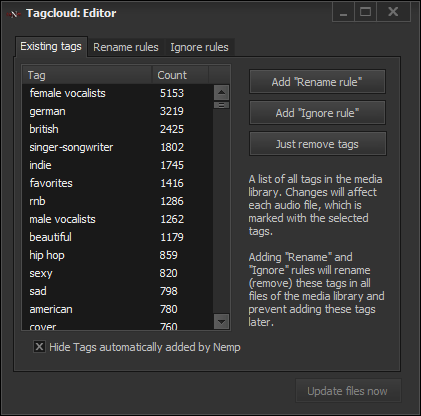
\includegraphics[width=0.8\textwidth]{tagwolken-editor_en.png}
%\caption{Der Tagwolken-Editor}
\label{fig_tagwolke}
\end{figure}

In the first tab \textbf{existing tags} you will find a listing of all, really all tags in the media library, from frequent like \emph{singer-songwriter} to exotic like \emph{songs die so gut sind das ich meiner oma ihr klein haeuschen zwar nicht verkaufen aber zumindest dafuer beleihen wuerde}\footnote{translates to: songs that are so good that I don't sell my grandmother's little cottage but at least lend it}, with which actually some titles at last.fm are filled.

You can create new rules by selecting one or more tags. A \emph{Rename rule} ensures that a tag is automatically changed to another tag. A \emph{Ignore rule} ensures that a tag is ignored and not saved. The function \emph{Remove tags} deletes the selected tags from the media library without creating a new rule. Nemp brings along a few of these rules by default.

 
\begin{beispiel} You have many titles with the tag \emph{Singer-Songwriter} in the media library, and a few more with \emph{Singer and Songwriter}. Both tags mean the same thing, but if they both stay, it makes browsing in the tag cloud more difficult.

So: Mark both tags and click on \emph{New rename rule}. Nemp then automatically proposes a new name, the tag with which most titles are marked. Of course, you can also choose a new name. If only one day is selected, there is of course no proposal for a new name.
\end{beispiel}

\begin{beispiel}
You regularly get extended tags automatically via last.fm. Some titles are often marked with \emph{favorites}, even if these titles are not necessarily your personal favorites.

So: Mark the tag \emph{favorites} in the list and click on \emph{New Ignore Rule}. When the automated tag search is called up again, Nemp will ignore this tag and will not mark the titles with it. But you should mark your own favorites with a different tag, otherwise you will get confused at some point.
\end{beispiel}

\begin{beispiel}
They have a large number of tags that only appear once or twice in the entire media library. These tags are usually not very useful, but an ignore rule for all these tags would be overkill.

So: Check all of these tags and click on \emph{Remove Tags}. Nemp will then simply remove these tags from all files without saving a new (relatively useless) ignore rule.
\end{beispiel}

After creating a new rule, it is also applied directly to the media library. Changing the tags within the Nemp database goes in no time. Changing the tags in the files themselves takes some time - usually a little longer than reading the files into the database. Therefore, the Nemp does not execute with every new rule, but only on direct instruction. To do so, click on \emph{Update files now}. If you don't do this, Nemp warns you that there are still inconsistencies between the data in the library and the data in the music files that should be fixed. If Nemp is then closed anyway, the changes are not saved in the files, and when the files are re-imported, the data in the library is overwritten with the data from the files.


\begin{tipp}
Double-clicking on a tag displays all titles marked with that tag in the Nemp main window. In this way you can display all the songs that are so good that some users of last.fm would not sell their grandma's little cottage but at least lend money for it.
\end{tipp}

The other two tabs list the rename and ignore rules. You can delete some rules here, but it is not possible to edit existing rules.

\section{Tools}
\label{sec_tools}

In addition to the basic functions \emph{play music} and the management of all music files in a \emph{media library}, Nemp offers a few more (more or less) useful tools.

\subsection{Scrobble with Nemp}
\label{sec_scrobbeln}
\begin{wrapfigure}[5]{R}{0.35\textwidth}
\centering

\includegraphics[width=0.35\textwidth]{lastfm_logo.jpg}
\end{wrapfigure}
Scrobbeling is an invention of last.fm - a social network on the internet with a focus on music. Scrobble means that what you're hearing now appears in your user profile on this page. Through the songs you hear over time, a taste of music crystallizes and you can use this network to find and get to know people with similar musical tastes. And then discover more bands that you might also like.

Nemp can scrobble.

\subsubsection{Scrobbler configuration}
First, you must allow Nemp access to your last.fm user profile. To do this, open the settings dialog and start the configuration. You have to be connected to the internet.

\begin{enumerate}
\item Start the configuration and click on \emph{Next}. Nemp requests a so-called token from last.fm, which is required for authentication in the following process. 

\item Click on \emph{Next} again. You will then be sent in your browser to the last.fm website, where you will need to log in with your account. After registration, you will be redirected to a page showing the Nemp logo. Click on \emph{Allow access} and switch back to Nemp. 

\item Click on \emph{Next} again (and directly again). Nemp can now retrieve your username and session key from last.fm using the token that you linked to your account by clicking on the allow button on the website. This key is stored in the Nemp configuration file (slightly encrypted) and is required for the Scrobble function. Nemp does not require your last.fm password itself.
\end{enumerate}

\subsubsection{Scrobbler activation}
Check the Scrobble settings under \emph{Scrobble this session} and click on \emph{accept} below. If you always want to scrobble, set a checkmark at \emph{Scrobble always}.
If scrobbling is active, the \inlinegraphics{scrobbler.png} icon will appear in the main window. 


\subsubsection{What is being scrobbled?}
Scrobbling runs in two phases. 

\begin{itemize}
\item The \emph{Now Playing} message. This is set at the start of a new title. In your profile then appears \emph{listens to (current title)}. 
\item The \emph{submission} message. This is sent at the end of a song if at least 50\% or 4 minutes of the song have been played. These titles will then appear in the history in your user profile. Titles that are too short (less than 30 seconds) are generally not scrobbled.
\end{itemize}

\subsubsection{Troubleshooting}

Sometimes there is a disruption in the connection to the service. Since Scrobbling is not a key feature of Nemp, the errors are simply ignored without displaying an error message. Nemp then terminates the scrobbling to avoid unnecessarily burdening the service. 

However, if updating the user profile is very important to you, these error messages can also be displayed in a message window when they occur. Otherwise, they are only displayed in the log area in the settings.

Possible sources of failure are
\begin{itemize}
\item No internet connection
\item A firewall blocks Nemp's communication with last.fm 
\item The session key is invalid. Then you have to repeat configuration steps 1.) to 3.) 
\item Your account is locked. Contact last.fm. 
\end{itemize}
If you believe that you have eliminated the cause of the error, you can start a new attempt by clicking on \emph{scrobble again}.

\subsection{The birthday mode}
\label{sec_birthday}
A small gimmick is the \textbf{birthday mode}. Here you can specify a time at which a previously defined song is to be played. Optionally, you can also specify a countdown title that will be played before the specified time.  The birthday song can be selected either via the Windows file selection dialog or via the currently marked title in Nemp. Playlist or media list does not matter, both are possible. The same goes for the countdown.\footnote{It may be that the concept behind it is not generally known. In Germany it is quite common to \emph{celebrate into} (\gf{reinfeiern in}) a birthday. This means that the party starts on the evening before the actual birthday and lasts until (long) after midnight. At midnight, a birthday song is usually sung (or bellowed), the gifts are presented and then the party continues. It's comparable to what you make into a New Year's Eve all over the world. Hence: Birthday mode.}

After the birthday song, the playlist can be automatically resumed or you can wait for further user input. In this case the player then remains silent until someone clicks on \emph{Play} again.

If birthday mode is active, the symbol \inlinegraphics{geburtstag.png} is displayed in the main window.


\subsection{The Nemp web server}

The Nemp web server offers the possibility to access the player from a browser via a network.

You activate the web server via the menu \emph{Tools - Nemp web server - Activate}. If the web server is activated, an \inlinegraphics{webserver.png} icon will appear in the main window. 

\begin{tipp}
Just try it out! Use your smartphone to access your WiFi and enter the IP address in the mobile phone browser. Alternatively \texttt{localhost} in the address line of the browser on the computer running Nemp.
\end{tipp}

\begin{center}
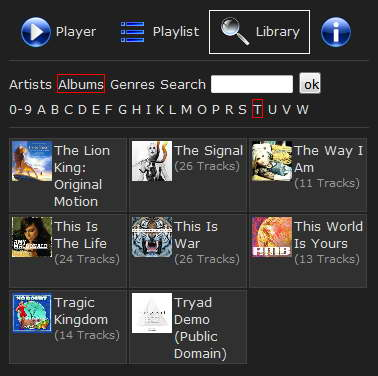
\includegraphics[width=0.5\textwidth]{webserver_screen.jpg} 
\end{center}

Depending on the chosen theme, a different range of functions is available. 

%\begin{hinweis}
%In contrast to previous versions, now only access from within the local network is possible. Access from outside is denied. The local network is recognized simply by the fact that the first three parts of the IP address must match.
%\end{hinweis}

\subsubsection{Configuration}
\label{sec_webserver}
\begin{itemize}
\item \textbf{Theme.} Selection of the layout and supported features. 
	\begin{itemize}
	\item In the theme \textbf{Default} all functions are available to all users (unless they are denied in the user authorizations). This theme uses Javascript.  
	\item The \textbf{No Javascript} theme offers (almost) all functions to all users, without the use of Javascript. Fast forwarding in the current title and volume control are not possible without Javascript. 
	\item In the theme \textbf{Party} there are limited functions for normal users. As administrator you have full access. 		
	\end{itemize}
Details on creating your own themes can be found in the separate documentation.

\item \textbf{activate the webserver at startup.}  \emph{default: Off.} Automatically activates the web server when Nemp is started.
\item \textbf{passwords for users and admins.} The web server has a rudimentary rights system. Administrators have extended access to the control of the player, which can be disabled for normal users. A user name and password can be assigned for both groups. This is useful for admin access, but not necessarily for user access.
\item \textbf{user rights}
		\begin{itemize}
		\item \textbf{Voting for files.} Users can click on \emph{Like} on entries in the playlist. Entries with many \emph{Likes} will slide up in the playlist and will be played preferentially (unless Nemp is in playback mode \emph{random playback}). 
		\item \textbf{Access to the media library.} Users can search for titles in the library and insert them into the playlist.
		\item \textbf{Downloading files.} Users can download titles to their device.
		\item \textbf{Remote control of the player.} Users can also access the player and pause, start, skip to the next track and change the volume. In addition, direct manipulation of the playlist is possible. You can then move or delete titles.	
		\end{itemize}			
\end{itemize}

\subsection{Keyboard display}

Since version 4.1, Nemp supports the display of the current title (and also the control) via the display of a keyboard such as the Logitech G15. 

\begin{center}
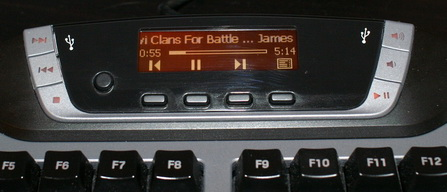
\includegraphics[width=0.5\textwidth]{g15.jpg} 
\end{center}

The support is not directly integrated in Nemp, but is realized via an additional tool. This tool uses the \emph{Nemp-API} to display information and provide rudimentary control of the player. 

The functionality of the multimedia keys on many keyboards is not affected by this. Of course, they work independently.

\begin{tipp}
If you have another keyboard with a display, you can theoretically write your own tool to support your keyboard. If you can code (or someone among your friends), please contact me for more information. E-mail: mail@gausi.de
\end{tipp}

\subsection{Automatic shutdown, sleep timer}

Nemp can shut down itself after a certain period of time and shut down or put the computer into hibernation. If the \textbf{Shutdown-Timer} is activated, the \inlinegraphics{shutdown.png} icon will be displayed in the player. 

If the set time has elapsed, a warning window will be displayed for 30 seconds to warn you that the PC will soon shut down. Of course, with the option of aborting the process. However, since this function is intended for falling asleep rather than working, no unsaved documents should be open any more. 

In these 30 seconds, the volume is slowly reduced and no new song is started to prevent the sleep process from being hindered by a sudden change in volume. 

\begin{hinweis}
For this, the sound scheme of Windows must be appropriately configured. Nemp does not prevent the possibly quite loud \emph{jingling} of Windows when the computer is shut down.
\end{hinweis}

\subsection{Playlist log}

A small feature request was a logfile for the player. Now here it is logged, when which track was played, if necessary with the remark \gf{aborted} if the title was not played back completely.

The definition of \gf{fully played} is the same as for scrobbling, i.e. at least 4 minutes or half of the title must be played. If a 3-minute track runs for 2 minutes, or a 1 hour mix for 5 minutes, then both tracks are considered \gf{played} and not \gf{cancelled}.

If you wish, this log file can also be saved automatically in order to to keep an overview of the titles that have been played in the past days. This is deactivated by default and must therefore be activated in the settings. There you can also set the amount of time you want to keep the logs (default: 7 days).


\section{Preferences, settings dialog}
\label{sec_einstellungen}

If Nemp has one thing in abundance, it's settings. In the course of time, there were always requests to ask whether you could do this or that. Much of it was then built in and has gradually increased the amount of adjustment possibilities. With version 4.7 some \emph{too} geeky settings were removed.

\subsection{General settings}
On starting Nemp
\begin{itemize}
\item \textbf{Begin playback on start.} \emph{Default: On.} When starting Nemp, start playing the music directly without having to click on \emph{Play}. This starts with the title that was last listened to.

\item \textbf{Remember last track position.} \emph{Default: On.} When starting Nemp, the last track played will be started at the position where Nemp was previously stopped and not at the beginning.

\item \textbf{If applicable: Start playback with new file.} \emph{Default: On.} If Nemp was started by double-clicking on an mp3 file, then this title will be played and not the title that was active when Nemp was last started.

\item \textbf{Switch to enqueued file (even if another track is already playing).} \emph{Default: Off.} If an mp3 file is double-clicked in Windows Explorer and passed to Nemp, the current playback is interrupted and the newly inserted title is played immediately.

\item \textbf{Allow multiple instances.} \emph{Default: Off.} Normally, Nemp should only run once, further starts will be blocked. With this option Nemp can be started several times.
\end{itemize}

Nemp auto updater
\begin{itemize}
\item \textbf{Automatically check for new versions of Nemp.} \emph{Default: Off.} Nemp can check at the specified interval whether a new version is available and then display an appropriate message. Download and \gf{installation} must be done manually.

\item \textbf{Notify on Beta releases.} \emph{Default: Off.} Also notify if there is no new stable version yet, but only a pre-release version in which more errors can occur than it should be in the final version.
\end{itemize}

Advanced skinning
\begin{itemize}
\item \textbf{Use advanced skinning system.} \emph{Default: On.} This uses an advanced skin system that draws window frames and many other control elements not in the Windows standard, but adapts to the skin if the skin supports it. Occasionally causes problems or crashes of Nemp. Deactivate if in doubt.
\end{itemize}

Advanced settings when starting Nemp
\begin{itemize}
\item \textbf{Show splash screen.} \emph{Default: On.} Shows the \emph{Nemp is starting}-window at startup.

\item \textbf{Start minimized.} \emph{Default: Off.} Nemp starts minimized without bringing the window to the foreground or displaying it.

\item \textbf{Stay on top.} \emph{Default: Off.} In separate window mode, the small player window can be kept permanently in the foreground as long as no other program wants to be \gf{first} in this respect.

\item \textbf{Load media library on start.} \emph{Default: On.}The most recently created media library is automatically loaded and displayed.

\item \textbf{Save media library on close.} \emph{Default On.} The current media library is automatically saved when Nemp is closed.
\end{itemize}

\subsubsection{Controls}
\begin{itemize}
\item \textbf{Use media keys, even if Nemp is in the background.} \emph{Default: On.} Nemp also reacts to play, pause, next title etc. by pressing the corresponding key on media keyboards, if Nemp is not the foreground window but only runs in the background.

\item \textbf{Use volume up/down keys for system-wide volume control.} \emph{Default: On.} By pressing the keys for \emph{volume up/down} on the media keyboard, the global volume is controlled. Otherwise, only the volume in Nemp is changed.

\item \textbf{Use keyboard display.} \emph{Default: Off.} Use Nemp to start a display application to show the current title in Nemp on the keyboard display. For the Logitech G15, Nemp comes with an application, for other keyboards you can program your own applications (theoretically).

\item \textbf{Hotkeys configuration.} \emph{Default: Off.} Nemp can register system-wide hotkeys to enable control when Nemp is in the background. This may interfere with the operation of other programs or their hotkeys.
\end{itemize}

The configuration of the Tab key is rather useless or strange, but it will not bother you either.

\begin{itemize}
\item \textbf{Tabstop at player controls.} \emph{Default: On.} The player keys can be focused with the Tab key and then activated by pressing \texttt{Enter}.

\item \textbf{Tabstop at tool buttons.} \emph{Default: Off.} The Tab key allows you to focus the toolbuttons for lyrics, covers, effects etc. using the Tab key.
\end{itemize}

\subsubsection{System}
\begin{itemize}
\item \textbf{Taskbar and/or Tray.} \emph{Default: Taskbar only.} Displays Nemp in the taskbar and/or as a small icon in the tray area and controls the behavior when minimizing. Hiding the taskbar entry is not recommended under Windows 7 and later.
\end{itemize}

\textbf{Notification of a deskband.} A \emph{deskband} is interesting mainly for users of Windows XP. This is an area in the taskbar that contains some controls. Nemp can install such a desktop (only on 32Bit-Windows) and configure it's behavior.

\begin{itemize}
\item Show deskband on start. \emph{(Default)}
\item Hide deskband on close. \emph{(Default)}
\item Show deskband on minimize.
\item Hide deskband on restore.
\end{itemize}

Nemp can react to it, if the PC is put into hibernation mode.

\begin{itemize}
\item \textbf{Stop player when system hibernates.} \emph{Default: On.} Stops the player, so when waking up the PC during login music playback \emph{not} is running.

\item \textbf{Reinitialize player engine on wakeup.} \emph{Default: Off.} Some systems require a re-initialization of the player if the PC is woken up from hibernation. Usually not necessary.
\end{itemize}



%%%%%%%%%%%%%%%%%%%%%%%%%%%%%%%%%%%%%%%%%%%%%%
\subsection{Viewing settings}
\begin{itemize}
\item \textbf{Columns in the media list.} A selection of the columns displayed in the lower list in the main window. Can also be selected by right-clicking on the column header. Also: Enable the additional display with cover and details next to the list.

\item \textbf{Sorting order} for the classic view and coverflow. In the Classic View, two sort criteria are specified, which can be combined as required. There are some preselections in the coverflow. You can also set special treatments for the coverflow for albums for which no cover has been found, or title compilations without proper metadata.

\item \textbf{Sorting.} \emph{Default: Off.} 
By clicking on a column header in the media list, you can sort the displayed list according to the corresponding criteria. This setting also applies if a new list is created and displayed using the overview lists (classic view, coverflow, tag cloud). This causes a small delay in the display. \emph{Therefore, ... }

\item \textbf{Skip sort on large lists.} \emph{Default: On.} ... when this option is activated, sorting very large lists can be deactivated to avoid excessive delays.

\item \textbf{Show marked files only from the current list.} \emph{Default: On.} When activated, clicking on the marker button next to the quicksearch field will show only marked files from the current selection. Otherwise, all marked files from the complete media library are shown.
\end{itemize}


\subsubsection{Party mode}

\begin{itemize}
\item \textbf{Amplification factor.} Option how much the player control should be increased when the party mode is activated.

\item \textbf{Block editing file information in the media list}. \emph{Default: On.} Prevents the title information from being edited by double-clicking or \texttt{F2} in the title list of the media library. The display of the detail window with extended editing options is always deactivated. 

\item \textbf{Black rating of current title}. \emph{Default: On.} Prevents you from changing the rating of the current title. 

\item \textbf{Password.} The optional password is required to exit Party mode. If necessary, it is displayed briefly when activated. If you forget your password, exit Nemp and restart. Party mode is then deactivated.
\end{itemize}


\subsubsection{Fonts}
The configurability of the fonts is a relic from the prototype Nemp, where I was mainly interested in showing what I can read from mp3-files. In the meantime I think these settings are not very useful and have set all values to \emph{Default: Off}.

\begin{itemize}
\item \textbf{Font size.} The general font sizes for the overview and title lists as well as the font style (normal, italic, bold) can be adapted to your own requirements.

\item \textbf{Change style according to channel mode.} Mp3 files can contain different numbers of channels. Some few are \emph{mono} (single-channel sound), most are \emph{stereo} (dual-channel sound). In stereo, there is still a distinction between \emph{Full stereo} (i.e. left and right channels are encoded separately) and \emph{Joint Stereo} (the second channel encodes only the differences to the first channel). Nemp can display the channel mode using the font style. Italics: Mono; Normal: Joint stereo; Bold: Full stereo.

\item \textbf{Change font size according to track length.} Longer titles are displayed larger, shorter ones smaller. Makes more trouble than it helps.

\item \textbf{Change font color according to bitrate.} Titles with a low bit rate (less than 160 kbit/s) are displayed in reddish color, titles with a high bit rate (more than 160 kbit/s) in green. The lower or higher the bitrate, the more intense the red or green will be. This is deactivated by the default skin of Nemp and has no effect there.

\item \textbf{Change font according to constant/variable bitrate.} The font can be used to indicate whether the title has been encoded with a constant or variable bit rate. In most cases, this is not a particularly interesting indication that requires special emphasis.
\end{itemize}

\subsubsection{Extended viewing settings}
\label{sec_extVis}
Some other settings that are less useful, but don't do any harm by being in.

\begin{itemize}
\item \textbf{Visualization.} \emph{Default: On, 25fps.} This refers to the bouncing bars in the main window. The update rate is only a reference value and not an exact specification. 

\item \textbf{Scroll title in taskbar.} \emph{Default: On.} Under Windows 7 and later less interesting, because only icons are displayed in the taskbar by default. Under XP, the name of the currently running program or open document is still displayed there. For longer titles, Nemp can scroll through this text (i. e. the currently running title). The speed is relative to the update rate of the visualization.

\item \textbf{Scroll title/path/details/lyrics in main window.} \emph{Default: On.} Same as above, except for the title display in the middle of the player.

\item \textbf{Show hints in the media list.} \emph{Default: On.} Displays hints with some details when hovering the mouse pointer over an entry in the media list for a short time.

\item \textbf{Show hints in the playlist.} \emph{Default: On.} Displays hints with some details when hovering over an entry in the playlist for a short time with the mouse pointer.

\item \textbf{Select full row in media list.} \emph{Default: On.} Clicking on an entry in the media list in the lower part of the window will select the entire row. Otherwise, only the clicked cell in the table.

\item \textbf{Not available metadata.} Not all mp3-files are always completely tagged with ID3 tags. Nemp can then display other information in the overview list instead. Which ones are useful also depends on how your own music collection is organized.

\item \textbf{Coverflow.} In some cases, the coverflow may cause some problems. The two settings here can be used to correct these in case of doubt.
\end{itemize}



%%%%%%%%%%%%%%%%%%%%%%%%%%%%%%%%%%%%%%%%%%%%
\subsection{Player settings}
In this section, you can set things that affect file playback.
\begin{itemize}
\item \textbf{Output devices.} Selection of sound cards detected in the system. Even if only one sound card is installed, there are occasionally several options available, but they are of little relevance. This selection is really only interesting if a second sound card is actually installed (or connected via USB) in order to select which card is used for the main output and what the headphones are used for listening. See section \hyperref[sec_headphones]{headphones}  for more information.

\item \textbf{Fading.} \emph{Default: On.} Allows a smoother transition between title changes. Can be disabled for some cases or actions.

\item \textbf{ReplayGain.} Settings for automatic loudness adjustment during playback.
Explanations about ReplayGain, the possible options and how it is implemented in Nemp can be found in the section \hyperref[sec_ReplayGain]{ReplayGain}. With this, the settings should be self-explanatory.

\item \textbf{Silence detection.} \emph{Default: On.} Nemp can detect silence at the end of a track and then, if necessary, initiates playback of the next track earlier in order to play the playlist without pauses. 

The threshold value specifies the volume at which Nemp should detect \emph{silence} that is to be skipped. Small values such as -10db cause the track to be aborted very early if the volume drops only slightly. Values of -40db or more do not jump to the next track until the volume of the track has been greatly reduced. The default value is -40db.

Since this detection is only started when the title is already running and can take a few seconds, it may happen that this function does not always work as expected for very short titles. \emph{Very short} means thereby less than 5-10 seconds, thus for the vast majority of cases that is no restriction. 

Silence at the beginning of a piece is not recognized and therefore cannot be skipped.
\end{itemize}


\subsubsection{Playlist}
\begin{itemize}
\item \textbf{Check files when loading a playlist.} \emph{Default: On.} Many formats for saving a playlist support only a few pieces of information about the titles. Nemp therefore scans the files when loading a playlist to get more information about the titles. For large playlists with several hundred files, this can take quite some time and can be deactivated if you want.

\item \textbf{Jump to next entry in cuesheet on \gf{next}.} \emph{Default: On.} Clicking on \emph{next title} will not play the next file, but only the next entry in the cue sheet, if there is one. Useful for CD-Rips, where the entire CD has been encoded into an Mp3 file.

\item \textbf{Repeat current entry in cuesheet on \gf{Repeat title}.} \emph{Default: On.} Repeats in the playback mode \emph{Repeat Title} only the current entry in the cue sheet, not the entire mp3 file.

\item \textbf{Remember track position when playing a song directly from the library.} \emph{Default: On.} If a song is played back in the library without inserting it into the playlist, the playlist will continue playing after the end of that song. If this option is activated, then it will also be at the exact position in the title where the playlist was previously interrupted. Otherwise, the last played song will be played in the playlist from the beginning.

\item \textbf{Default actions.} 
Specifies the action to be performed when double-clicking an entry in the media list, or whether and where the selected title is to be inserted in the playlist.

\item \textbf{Stop headset when switching to another tab} \emph{Default: On.}
\gf{Another tab} refers to the other elements in this area, i.e. cover, lyrics, effects and equalizer. If you switch to another display, playback in the headphones is interrupted.

\item \textbf{Delete completely played tracks from the playlist.} \emph{Default: Off.}
If desired, finished tracks are removed from the playlist, which can be disabled if you have used an action such as pause, stop or fast-forward during playback.

\item \textbf{Mix playlist after last track}. \emph{Default: Off.} 
When the playlist has been played back completely, the playlist is then shuffled, i. e. all tracks are randomly re-ordered. This option does not work for random playback of the playlist.
\end{itemize}

\subsubsection{Random playback}
\label{sec_random}

What we humans generally perceive as \emph{by chance}, it is usually not that. And that which is actually (more or less) random, is often felt as \emph{not} random. For example, in an actual \emph{random} playback of the tracks in a playlist with 16 tracks, it is very likely that you have to listen to 40 tracks and more until every track has been played at least once. On the other hand, this leads to the fact that some songs are played very often. Such behaviour is not an error in \emph{programmed} randomness, but an inherent characteristic of that which constitutes randomness.

\begin{itemize}
\item \textbf{Really random ... avoid repetitions.} \emph{Default: quite random.} In order to achieve a perceived random play back in Nemp, something is tricked. The control can be used to set how long a played track should be locked for replay. If an entry in the playlist that has been played \gf{recently} is randomly selected, the next title that hasn't been played recently will be played instead. This is defined by the number of titles in the playlist. If the slider is exactly in the middle, then a playlist with 16 songs has to play at least 8 tracks (50\%) before the title can be played again randomly.

A manual selection of a track that has been repeated many times before is of course always possible.

\item \textbf{Weighted randomness.} \emph{Default: Off.} 
Normally, each title in a playlist has the same chance of being selected for random play. In the Urn model, which is probably known to everyone from school or drawing of lottery numbers, each title is included exactly once, and then a title is randomly taken, which then is played.

But you can also - to stay in the lottery example - put some numbers into the urn several times. For example, if the 42 would be in the urn not only once, but 100 times, then you can easily imagine that the 42 would be taken at almost every drawing.

Nemp can do something similar with the random playlist playback based on the ratings of the titles, with adjustable weights for each rating. A weight of 60 means that a title is thrown into the urn 60 times, from which a title is drawn randomly. The probability that this title will be played back is correspondingly higher than that of a title that only weighs 10 or even 1. 

A weight of 0 means that this title cannot be selected randomly at all. Nevertheless, such titles can be played back in the playlist by \gf{random}. Namely, when they are taken as a fallback option, if the random slider in the other option is moved further in the direction of \emph{avoid repetitions}.
\end{itemize}

These two options clash a little bit, and there may be unexpected effects. That strongly depends on how often individual assessments have been assigned, how much weights are chosen, and how much at random \gf{decided} to avoid repetitions.

The button \textbf{Count ratings} evaluates how often individual ratings are found in the playlist or the entire media library. This gives you an overview of whether the weightings selected are meaningful at all or, in most cases, are empty, because the corresponding evaluations do not occur at all.

\subsubsection{Web radio}
The web radio functions in Nemp are quite rudimentary. Nemp supports web radio, but the focus is not on it.

\begin{itemize}
\item \textbf{Parse stream playlist.} In the small files downloaded from web radio sites on the Internet, several URLs can be listed, which usually all send the same but in different qualities. Nemp can either parse this file and offer all stations to play, or only one entry from which the playback engine selects a suitable station on its own.

\item \textbf{Recording settings.} Nemp can also record webstreams in mp3 format. Here you can set where the recordings should be saved, how the files should be named, whether a separate subfolder should be used for each station, and whether and how the files should be cut.

Beginning a new file when changing the title depends on how exactly the sender sends the meta information. This works very well for some stations, badly for some, and practically not at all for others.

As an emergency option, you can then cut after a certain time or when a certain file size is reached. These crop marks are only approximate values. The file sizes and title lengths may differ slightly from the indicated ones.

Streams that are not encoded in Mp3 format cannot be recorded.
\end{itemize}


\subsubsection{Effects}
\begin{itemize}
\item \textbf{Reset equalizer/effects.} Depending on the setting selected at this point, the effects and equalizer settings will be forgotten when Nemp is restarted and reset to the default setting or not. The default setting retains the equalizer setting, but resets the effects back to \emph{off}.

\item \textbf{Jingles.} Pressing the \texttt{F9} key (and holding it down) will play an additional title. This playback is stopped immediately when the button is released. The volume of the actual playback can be reduced.

\item \textbf{Walkman mode.} A silly little gimmick. Some \gf{older} people might still know the Walkmans (or \emph{portable cassette players} from other brands). They started to wobble when the battery was low, as the tape no longer ran at constant speed. 

Nemp can simulate this behavior. If Nemp is running on a laptop that is not connected to the power supply, playback will no longer run at constant speed. The effect becomes stronger and stronger as the state of charge decreases. This is actually counterproductive, since it will cost more computing power. But at least it is more noticeable when the battery is weakening and needs to be charged.
\end{itemize}


\subsubsection{Birthday mode}

See section \hyperref[sec_birthday]{Tools - The birthday mode}.


\subsubsection{LastFM}

See section \hyperref[sec_scrobbeln]{Tools - Scrobble with Nemp}.

\subsubsection{Web server}
See section \hyperref[sec_webserver]{Tools - The Nemp web server}.


\subsubsection{Extended player settings}
\begin{itemize}
\item \textbf{Buffer size.} \emph{Default: 500ms.} In some cases, a larger buffer can avoid jerky jerks if it is not always possible to read from the source (hard disk, USB stick, CD) quickly enough. This will also effect changes to the equalizer settings or effects with a longer delay.

\item \textbf{Floating-Point channels.} So-called floating point channels provide better audio quality, but can sometimes cause problems. Nemp can automatically detect whether this feature is supported by the system. In case of problems: Switch off.

\item \textbf{MIDI playback.} For playing MIDI files, so-called SoundFonts are required. Since Nemp does not focus on MIDI files, these (often very large) sound font files are not included. Some SoundFont files can be downloaded 
\href{http://www.un4seen.com/download.php?x/ChoriumRevA}{here} or
\href{http://www.un4seen.com/download.php?x/ChoriumRevA}{here}.
If you copy the sf2 file contained in these archives to the bass-subfolder and restart Nemp, this SoundFont file will be used if you have not explicitly selected another one. 

\item \textbf{Safe playback.} \emph{Default: Off.} An setting associated with variable bitrate files. For such files, it may be necessary to scan the entire file for accurate scrolling. This happens in the default setting after the title is started, which can cause problems (but usually does not). With \emph{safe playback} the file is completely scanned before the playback starts. However, this will delay the start of playback noticeably for larger files.
\end{itemize}



%%%%%%%%%%%%%%%%%%%%%%%%%%%%%%%%%%%%%%%%%%%%%
\subsection{File management}
The original core feature of Nemp was the file management, which is still a central element.

\begin{itemize}
\item \textbf{Directories.} Nemp can manage a list of directories that are scanned for new files every time Nemp is started. This is only useful if the media library is growing regularly and often new files are added. With more static music collections, it makes more sense to search for new files manually only when needed.

Since Nemp 4.9 you can also search for missing files when starting, which are then automatically removed from the Media Library. If files are on a drive that is currently unavailable, the files remain in the library. If a new drive is connected while Nemp is running, the search for unavailable files for this drive is repeated.

\item \textbf{File types for the media library.} Specify which file types (identified by the file extension) you want to include in the library. By default, everything that can be played is inserted. This unfortunately also includes mp4 files, but these are usually video files. Nemp also plays these files (mostly) but only audio, without video.
If movies and music are stored in different directories, this is no problem. Otherwise exclude the file type mp4 from the media library if necessary.

\item \textbf{Scan files in playlists.} \emph{Default: On.} 
Playlists are also included in the media library, even if they are only vidibld in the \emph{classic view}. The individual files in it are not added to the media library separately again. Some metadata may be missing for viewing these playlists when you browse them. 

For rather short lists, fast scanning is possible. If many large playlists have been created, this can cause noticeable delays in the display and can therefore be deactivated.
\end{itemize}


\subsubsection{File types registration}
If you want to use Nemp as the default music player, you can configure the corresponding system settings here.
\begin{itemize}
\item \textbf{Enqueue as default action.} Ensures that new files (or playlists) are inserted into the currently active playlist without deleting the current playlist. Otherwise, the current playlist will be deleted first, and then the newly selected title will be inserted.
\item \textbf{Context menus on directories.} Adds the \emph{Play in Nemp} and \emph{Enqueue in Nemp} entry to the folder context menu to play entire directories by right-clicking with Nemp.
\end{itemize}
The changes on this page of the settings must be confirmed by a separate click on the button \emph{Apply changes}. Under Windows 10, Windows may want to confirm these settings again. Then select Nemp as the \emph{default app} for music.

\subsubsection{Metadata}
\label{sec_metadaten}
Metadata are additional information in the music files, often referred to as \emph{ID3 tags}. ID3 tags are actually only the special case for Mp3 files, which is best known due to the widespread use of this format.
\begin{itemize}
\item \textbf{Allow quick access.} \emph{Default: Off.} This setting is queried via the \emph{Nemp-Wizard}, because I think it makes sense - but the files are changed very quickly. A click on the asterisk rating is sufficient to effect a change in the file, which may conflict with your backup strategy and cause unnecessary additional effort during the backup.

If this option is enabled, some metadata such as interpet, title, or album can be changed directly from the media list display.


\item \textbf{Ignore lyrics.} \emph{Default: Off.} With very, very large music collections, Nemp reaches certain technical limits. So far there exists Nemp
only in a 32-bit version, and the usable memory is limited to 2GB. If 1 million songs contain lyrics with 1000 characters each, 1GB is already used to keep all lyrics in memory that are rarely or never used.

Therefore (since Nemp 4.9) the collection of lyrics in the media library can be stopped for such cases. All previously saved lyrics are removed from the library and are therefore no longer available for searching. Of course, the texts in the ID3 tags are retained, and they are still displayed when you play a title or open the detail window.

\item \textbf{Resolve inconsistencies when entering new tags.} \emph{Default: On.} Inconsistencies can occur when entering new extended tags for the tag cloud. These are minor inconsistencies such as duplicates of a tag, or more severe ones such as inconsistencies with the Ignore- and Rename-rules defined in the tag cloud editor. Nemp can automatically resolve these inconsistencies by deleting (or not creating) duplicate entries and applying the Ignore- and Rename-rules to the user input.

\item \textbf{Automatic rating and play counter.} Nemp can also count how often you listen to which files. This information is stored in the media library and - if quick access to metadata is allowed - also in the file's metadata. 

If you do not allow quick access to metadata when selecting this option, the evaluation and playback counters may be lost when the media library is re-loaded.

Automatic rating increases the rating if a title has been played back completely. It is decreased when a song is cancelled. Both are optional.

	\begin{itemize}
	\item \emph{Abgespielt} A song is \emph{played} if it is played at least halfway, or at least 4 minutes of it.
	\item A title is considered \emph{canceled} if it has not been \emph{played} and the player has not been stopped. So if you click on \emph{Stop} after a few seconds or stop Nemp completely, this will not have a negative effect on the rating of the title just started. Only if you select a new song during playback.
	\end{itemize}
	
The change in the rating is not immediately visible on the asterisk scale. Internally, the evaluation runs from 1 to 128, which is rounded to half asterisks for the display.

\item \textbf{CD-Audio.} When playing an audio CD, Nemp can query the CD database on the Internet to display the title information.

\item \textbf{Unicode.} This is a very complex subject, but I must briefly address it here to explain this option. The basic problem is nicely summarized in this picture.
\begin{center}

\includegraphics[width=0.25\textwidth]{encoding.png} 
\end{center}
For non-German speakers: This should read \emph{Schei� encoding}, (\emph{shit encoding}). However, the letter \gf{�} cannot be read due to incorrect coding.

The ID3 tags contain many, many bytes. These are numbers between 0 and 255, and if there is a \emph{text} in a file, these numbers are interpreted as letters and displayed accordingly. At \gf{normal} letters A-Z and a-z there are no problems in general. Umlauts are already on the way. And when you then change the alphabet, e.g. to Cyrillic, Greek or Hebrew, it becomes difficult. 

All existing characters get their own unique number via \emph{Unicode}. Most of them (apart from the Latin alphabet) have a number (obviously) beyond 255, but if a byte only has a maximum value of 255, you have to think about how to encode these characters correctly.

The most useful method for this are the encodings \emph{UTF-8} or \emph{UTF-16}. Practically all characters can be coded with it. But if a program doesn't understand UTF-8, you get effects like in the picture.

Another method are the \emph{ISO-8859-standards}. You agree on a certain range of the Unicode number space and interpret the values between 0-255 differently. Depending on the interpretation, a Cyrillic letter is displayed, a Greek, Hebrew, Thai, or anything else. However, this only works if you only exchange files with people who have agreed on the same ISO 8859 standard.

And now we come back to the ID3 tags. There is no space for UTF-8 or UTF-16 in the very simple ID3v1 tag, nor is there any space for marking which ISO-8859 standard is used. This can result in titles with characters that do not appear in the Western European character set not being displayed correctly. And not correct often means: Completely absurd signs.

The clou is: These titles usually have corresponding characters in the file name - and here Nemp can start with a trick.

\textbf{Automatically identify the used character set.} \emph{Default: On.} If no UTF-8 or UTF-16 is used, Nemp tries to use the file name to determine which character set was probably used when writing the metadata, and interprets the values according to this character set.

Of course, this does not always work properly. But it's a significant improvement over what some other players display in such cases.
\end{itemize}


\subsubsection{Cover and Lyrics}
\label{sec_coversettings}

In this section, you can configure the search for covers and lyrics for the library. The default setting for the cover search is the following search behavior, which turned out to be very reliable in extensive tests.

\begin{itemize}
\item Search in the directory itself
\item Search in a subdirectory named \emph{cover} 
\item Search in the parent directory (if there are not too many files/folders in it) 
\item Search in a \gf{sister directory} named \emph{cover} (if there are not too many files/folders) 
\end{itemize}

The idea behind it are the following cases, in which the matching picture to the songs is successfully found.

\begin{tabular}{|l|l|l|l|}
\hline 
\begin{minipage}{2.6cm}
\small
\begin{verbatim}
c:\aAlbum\
   Track1.mp3
   Track2.mp3
   front.jpg  
\end{verbatim}
\end{minipage}
 & 
\begin{minipage}{2.8cm}
\small
\begin{verbatim}

c:\aAlbum\
   Cover\
     front.jpg
   Track1.mp3
   Track2.mp3
\end{verbatim}
\end{minipage} 
 & 
\begin{minipage}{3.35cm}
\small
\begin{verbatim}
c:\aSampler\
   CD 1\
      Track1.mp3
   CD 2\
      Track2.mp3
   front.jpg 
\end{verbatim}
\end{minipage} 
& 
\begin{minipage}{3.35cm}
\small
\begin{verbatim}

c:\aSampler\
   CD 1\
      Track1.mp3
   CD 2\
      Track2.mp3
   Cover\
      front.jpg 
\end{verbatim}
\end{minipage} \\ 
\hline 
\end{tabular} 

\begin{itemize}
\item \textbf{Try to get missing covers from last.fm} \emph{Default: Off.}
In addition, Nemp can search for missing covers on the internet at last.fm. In order not to start an Internet query every time a cover is displayed, unsuccessfully searched covers are saved. After some time Nemp tries to find the cover again. The idea behind this is that the last.fm database may not yet be up to date with new albums. If the cover cannot be found for a longer period of time, the search for this cover will be stopped completely.

The button \emph{Clear cache} deletes the information about unsuccessfully searched covers and Nemp will start searching for them again.

\item \textbf{Default cover.} Selection of a custom default cover in case Nemp cannot find a cover for an album or title. Covers already displayed in the player are not updated until the cover is reloaded, i. e. when a new song is started or when the coverflow is scrolled through.

\item \textbf{Online search for lyrics.} Here you can configure which online sources with which priority should be used for the search for lyrics. Standard is LyricWiki, optionally ChartLyrics can be used as fallback. In most cases, however, LyricWiki will achieve better results.
\end{itemize}

\subsubsection{Search settings}
A huge media library is of little use if you can't find anything in it. Therefore, Nemp contains a quite strong search function.

\begin{itemize}
\item \textbf{Accelerate search.} \emph{Default: On.} As with many problems in computer science, different methods can be used for text searches. You can often save time by using more memory space. When the search is accelerated, Nemp uses more memory to speed up the search. 

With very, very large music collections (i.e. several hundred thousand titles) a problem can arise here, since Nemp is so far only available in a 32-bit version and therefore the usable memory is limited to 2GB. If this occurs, Nemp will automatically disable this option. However, this can still lead to undesired behavior or even a crash.

\item \textbf{Including filenames/comments.} For accelerated search, a copy of all text information is created, which can be accessed more quickly. Depending on the structure of the music collection, it may be useful to include file names or comments in this copy. 

Since the filename also contains the complete path, this option can be useful if, for example, the self compiled sampler \emph{Vacation 2016 in Barcelona} is located in a folder. Then a search for \emph{Barcelona} will find this folder, even if the ID3 tags are not set accordingly.

Including the comments may lead to confusing search hits, if the searched term does not appear in the artist or title, but only \gf{hidden} in the field \emph{comment} of the ID3 tag, which is often used for incidental information such as codec settings. However, if you use the comments for useful information, you should also include them in the quick search.

\item \textbf{Accelerate lyrics search.} \emph{Default: Off.} A little bit hidden is the function to search for lyrics. This is not possible via the quick search, but only via the extended search, accessible via the menu. Here the same procedure can be used to speed up the search. For large music collections, where most of the lyrics are also available, the memory consumption increases significantly. 

If the lyric search is often used, you can activate it, but usually this is not necessary.

\textbf{Important: }If the \gf{Ignore lyrics} option has been activated in the metadata settings, the lyric search does not work at all. Nemp then ignores the texts stored in the ID3 tags and does not include them in the media library. The fact that the texts are still displayed during playback and in the detail window does not change this. Because the information displayed in this way is always also synchronized  with the information in the file stored data.

\item \textbf{Quick search.} In my opinion, the quick search in the main Nemp window is really fast. The results are displayed (almost) instantly even in very large music collections. By default, even while typing - with each additional character the hit list is further restricted.

If no matches were found for a search term, this may also be due to typing errors - in the search term or in the metadata of the files, or to inconsistencies such as \emph{P!nk} or \emph{Pink}. Nemp therefore also supports a fuzzy search, which is performed by default only when pressing the \texttt{Enter} key. On newer computers, however, the fuzzy search also works without any noticeable delay during typing, if there are not too many files in the media library.

\item \textbf{Change coverflow according to results.} In addition to presenting the search hits in the list, the coverflow can also be restricted to the search results. The search hits can then be further refined via the coverflow.
\end{itemize}

\newpage

\section{The Nemp Skin System}

Nemp's skin system is a self-made one, and has changed over the years. With the flexible layout of the main window (since version 4.11) some options of the previous skin system don't make sense anymore, but other things have been added.

A \gf{Nemp Skin} basically consists of three parts
\begin{itemize}
\item a whole series of images (for the background and buttons)
\item a configuration file \texttt{skin.ini}
\item optionally a \texttt{.vsf} file. This file is a so-called VCL styles file, which can be used to give windows a different look in Delphi programs.
\end{itemize}

\subsection{Images and graphics}

All images may be available as PNG, JPG or BMP. Nemp automatically selects the existing file extension. For background images JPG is recommended, for other images PNG.

\subsubsection{Background images}
The biggest changes with version 4.11 were here. The main reason for this is the now flexible layout of the main window. \emph{One} fixed background image apart from the control panel, which may even be aligned to it, makes little sense now. Instead there are now some of the large areas with separate background images, which can be aligned in several ways. 

\begin{itemize}
\item \texttt{player}. Except for the size, it's the same as before. Used for the part with the Play/Pause/Stop/Volume buttons.
\item \texttt{ControlProgress}. Same height as \texttt{player}, but the width is variable here (optionally tiled). For the part with the progress bar.
\item \texttt{ControlSelection}. For the narrow part to select main and headphone controls.
\item \texttt{ControlCover}. For the background of the small cover in the control panel.
\item \texttt{main}. Background for the remaining area of the window, is overwritten by the following three images for the subareas, if necessary.
\item \texttt{BackgroundBrowse}. Appears in the tag cloud and \gf{classical view}. Not currently in coverflow.
\item \texttt{BackgroundMedialist}. For the listing of titles in the media library
\item \texttt{BackgroundPlaylist}. Background image for the playlist.
\item \texttt{Win7PreviewBackground}. Background of the preview in the taskbar (Windows 7 or higher).
\end{itemize}
The image file \texttt{extendedplayer} is not used any more.

\subsubsection{Button graphics}

The images for buttons consist of several very similar individual images. Basically, all these images have five columns, i.e. five images next to each other. Of these five, only four are still in use:
\begin{itemize}
\item default state
\item MouseOver, i.e. you point with the mouse to the button
\item (unused)
\item MouseDown, d.h. you click the button
\item deaktiviert, i.e. the button is inactive and cannot be clicked.
\end{itemize}

Some buttons have different states, e.g. the Play/Pause button or the one for changing the playback mode. For each of these states there is a row in the graphics. 

\begin{itemize}
\item \texttt{BtnPlayPause}: Two rows for Play and Pause
\item \texttt{BtnStop}: Two rows. The second row is for the state \gf{Nemp will stop after the current title}
\item \texttt{BtnRandom}: Four rows for the for playback modes
\item \texttt{BtnRecord}: Two rows for start and stop recording
\item \texttt{TabBtnBrowse} and \texttt{TabBtnTagCloud}: Three rows. The first two for \gf{selected} or \gf{not selected}. The third one displays a warning if the ID3 tags of some titles have been changed at a significant position, and therefore the preselection lists or tag cloud should be rebuilt. Since this takes a few seconds, it does not happen automatically after editing individual titles.
\item \texttt{TabBtnMarker}: Five rows for the individual colored markings.
\item \texttt{TabBtn*}: Two rows each for \gf{selected} or \gf{not selected}.
\end{itemize}

\subsubsection{Additional graphics}
The rest of the graphics should be self-explanatory. Here is just a note about \texttt{ListenBilder} and \texttt{MenuImages}: These are used for symbols in the lists or for the symbols in the menus. However, not all single images are used anymore. The unused ones are still included for reasons of downward compatibility.

\subsection{The VSF file}

Some elements can't be adjusted by image files, e.g. the scrollbars, the window borders and the menus. Delphi offers VCL styles for this purpose (VCL stands for \emph{Visual Component Library}). A Nemp skin can use these style files to visually adjust the rest of the main window and the other windows. This part can always be activated or deactivated in the menu via \emph{use advanced skinning}.

\subsection{The configuration file  \texttt{skin.ini}}

In the configuration file \texttt{skin.ini} mainly colors and the positions of the buttons are defined, as well as some other options for the skin.

Since Nemp 4.11 has changed the size of the control panel on which most buttons are positioned, old data there may be inappropriate. Therefore, version 4.11 will ignore these entries as long as the \texttt{skin.ini} is not explicitly designed for this version. This is done via the following section in the file.
\begin{verbatim}
[Skin]
Version=4
\end{verbatim}

The file is divided into blocks as usual for ini files. A new block starts with \texttt{[section]}. The individual options in the block are then listed as \texttt{Descriptor=Value}. For Boolean variables (True/False) \texttt{1} means \gf{True} and \texttt{0} \gf{false}.

\subsubsection{\texttt{[Background]}}

Some options for the background images
\begin{itemize}
\item \texttt{HideBackgroundImage<..>}:  Don't use the background for that area, even if there is a matching file in the skin folder.
\item \texttt{TileBackground<..>}: Tile the backgound. If no tiling is used, the remaining area will be filled with the background color.
\item \texttt{AlignBackground<..>}: Alignment of the background images. The different values mean
\begin{enumerate}
\setcounter{enumi}{-1}
\item left-center
\item right-center
\item aligned to the control panel (you can use \texttt{PlayerPageOffsetX/Y} additionally)
\item left-top
\item right-top
\item left-bottom
\item right-bottom
\end{enumerate}
The value \texttt{2} is a relic from the previous versions and is no longer really meaningful with the variable design of the main window.
With \texttt{PlayerPageOffsetX} and \texttt{PlayerPageOffsetY} an offset for the main background image \texttt{main} can be specified, if it is to be aligned at the control panel.

\item \texttt{PlayerPageOffsetX, PlayerPageOffsetY}: Offset for the background image.

\item \texttt{AlignControlProgressDisplay}: Alignment of the background image for the progress display in the control panel.
\end{itemize}

\subsubsection{\texttt{[Options]}}
Some general skin options
\begin{itemize}
\item \texttt{UseSeparatePlayerBitmap}: use the separate background images for the control panel.
\item \texttt{DrawTransparentLabel}: Draws various labels (e.g. title information in control panel) with transparent background.
\item \texttt{DisableBitrateColors<..>}:  Nemp can display titles with high or low bit rates in different colors (see \hyperref[sec_einstellungen]{Viewing settings}). With these options this can be deactivated for the skin.
\item \texttt{Disable<..>Scrollbar}: Hides the scroll bars in the respective part.
\item \texttt{UseBlendedSelection<..>}: Draws the marked elements in the lists in the respective part with a semitransparent color for better readability. Transparency value: \texttt{blend factor<..>}, color \texttt{Tree\_(un)FocussedSelectionColor} in the corresponding section.
\item \texttt{UseBlended<..>}: Also uses a semi-transparent background for unmarked elements.  Transparency value: \texttt{blend factor<..>2}, color \texttt{Tree\_Color} in the corresponding section.
\item \texttt{HideMainMenu}: Hides the main menu.
\item \texttt{UseDefaultListImages, UseDefaultStarBitmaps}: Use the default graphics instead of the skin graphics.
\item \texttt{BlendFaktor<..>}: Transparency value for selected entries in the lists. \texttt{0} is completely transparent, \texttt{255} completely non-transparent.
\item \texttt{BlendFaktor<..>2}: Transparency value for non-selected entries in the lists.
\item \texttt{ButtonMode, SlideButtonMode}: Specifies how the buttons are to be drawn. \texttt{0} is Windows standard, \texttt{1} Windows standard, but with the skin graphics, \texttt{2} completely drawn by the nemp skin. \texttt{Slidebuttons} are the sliders for progress and volume.
\item \texttt{DrawGroupboxFramesMain}: Draw a border around some elements.
\item \texttt{UseAdvancedSkin}:  Use the advaced skin system with the \texttt{vsf}-file.
\item \texttt{AdvancedStyleFilename}: Filename of the \texttt{vsf}-file.
\end{itemize}

\subsubsection{\texttt{[Colors]}}
Definition of various general color values. All values are given in the format \texttt{\$00ggrrbb}, i.e. G-R-B. In graphics programs, the order R-G-B is usually used. Here, the order of the hexadecimal values must be reversed.
\begin{itemize}
\item \texttt{FormCL}: Background color for the main window.
\item \texttt{LabelCL}: Font color of the labels in the main window
\item \texttt{LabelBackGroundCL}: Background color of the labels if they are not to be drawn transparently.
\item \texttt{Spec<..>CL}: Font color of some special labels in the main window
\item \texttt{SpecPenCL, SpecPen2CL, SpecPeakCL}: Color values of the visualization, i.e. the jumping bars. A color gradient is created between \texttt{SpecPenCL} and \texttt{SpecPen2CL}, \texttt{SpecPeakCL} is for the small peak strokes, which sink more slowly.
\item \texttt{GroupboxFrameCL}: Color for the border of some elements.
\item \texttt{MemoBackGroundCL, MemoTextCL}: Background and font color of the lyrics display in the main window.
\item \texttt{ShapeBrushCL, ShapePenCL, ShapePenProgressCL, ShapeBrushProgressCL}: Color and frame color of the progress bar.
\item \texttt{Splitter1}: Color of the sliders in the main window for changing the size of the individual areas.
\item \texttt{PlaylistPlayingFileColor}: Frame color for the current title of the playlist.
\item \texttt{MinFontColor, MiddleFontColor, MaxFontColor}: Colors for displaying different bit rates. The system is based on the possible bit rates for mp3 files. \texttt{MiddleFontColor} is used for 160kbit/s, the maximum value for 320kbit/s (or more). 
\item \texttt{MiddleToMinComputing, MiddleToMaxComputing}: The possible values \texttt{0}, \texttt{1} and \texttt{2} indicate the type of gradient: square, linear or square-rooted.
\item \texttt{Preview<..>Color}: Color values for the preview in the Windows taskbar.
\end{itemize}

\subsubsection{\texttt{[<..>Colors}]}

The four section \texttt{[ArtistColors]}, \texttt{[AlbenColors]}, \texttt{[PlaylistColors]}, \texttt{[MedienlisteColors]} define some colors in the lists.

\begin{itemize}
\item \texttt{Tree\_Color}: Background color.
\item \texttt{Tree\_FontColor}: Font color.
\item \texttt{Tree\_FontColorSelected}: Font color of the selected items.
\item \texttt{Tree\_UnfocusedColor}: Font color of the selected items, if the list is not focussed.
\item \texttt{Tree\_HeaderBackgroundColor}: Background color of the header.
\item \texttt{Tree\_HeaderFontColor}: Font color of the header.
\item \texttt{Tree\_BorderColor}: Color of the little gap between columns in the header.
\item \texttt{Tree\_DropTargetBorderColor, Tree\_DropTargetColor}: Colors for Drag \& Drop
\item \texttt{Tree\_FocussedSelectionBorder, Tree\_FocussedSelectionColor}: Colors for selected items in the list
\item \texttt{Tree\_UnfocusedSelectionBorderColor, Tree\_UnfocusedSelectionColor}: Colors for selected items in the list, if the list is not focussed.
\item \texttt{Tree\_SelectionRectangleBlendColor, Tree\_SelectionRectangleBorderColor}: Colors of the selection rectangle for multiple selection by mouse.
\end{itemize}


\subsubsection{\texttt{[Buttons]}}

Position and size of some controls. The meaning of the individual values should speak for itself. 

\textbf{Reminder:} The positions defined here \texttt{left, top} are only used in Nemp 4.11 if the \texttt{skin.ini} also contains the section \texttt{[Skin]} with a suitable version information:
\begin{verbatim}
[Skin]
Version=4
\end{verbatim}
This is necessary so that skins created for Nemp 4.10 (or earlier) do not place the buttons outside the visible area.

\newpage

\section{Nerd stuff}

Nemp contains some more hidden and/or wacky features. Some of them have been requested  over time, others are historically determined, others are just for fun. I would like to draw your attention to a few things here.

\begin{itemize}
\item \textbf{The Nemp-API.} Originally, Nemp was just an Mp3-manager with a remote control for Winamp. The Winamp API was used for this purpose, which allows other programs to send commands to Winamp and read data from it. Nemp has basically copied this API and extended it a little bit. If you are interested, you can examine the file \texttt{src/common/NempAPI. pas} in the source code folder or use it in your own projects.

The Nemp Deskband for Windows XP and the display app for the Logitech G15 included with Nemp work with this API.

\item \textbf{command line parameter.} Nemp supports a few parameters for the command line. Some of them are used for the function \emph{Play in Nemp} respectively \emph{Enqueue in Nemp} in the Windows Explorer. Another hidden function is the parameter \texttt{/close}. A few years ago, a user requested a method to terminate a running instance of Nemp from the command line. First there was the small add-on program \textit{NempClose. exe}. In Nemp 4.8 this can be done by calling \texttt{./nemp.exe /close}. This terminates the current instance.

\item \textbf{Easteregg for Entwickler-Ecke.de.} Originally Nemp was published in the Delphi forum on \href{https://entwickler-ecke.de}{entwickler-ecke.de}. There I also worked as a moderator for several years and took part in the traditional Advent Lottery. One of these puzzles revolved around an mp3 file whose audio data was actually the source code of a brainfuck program that outputs a Christmas carol during execution. Nemp recognizes this special file, extracts the Brainfuck program, executes it and plays the hidden song. By the way, it was this one: Allison Crowe - Silent Night (video on \href{https://www.youtube.com/watch?v=zERIiMe1tNE}{youtube}).

\item In addition, there is a backdoor to quit the party mode, i.e. an admin password stored in the source code, with which you can always quit this mode.
\end{itemize}

\newpage


\section{Version history}

The following is a summary of the new features in the individual versions - from the current version to the very first version of this program, which at that time was not even a player. In this section you will find the main new features and noteworthy bugfixes, but not a complete list of all changes.

\subsection*{Version 4.12.1, October 2019}
\begin{itemize}
\item fixed possible exception while scanning for new files
\end{itemize}

\subsection*{Version 4.12.0, October 2019}

\begin{itemize}
\item Smoother scanning of metadata: the player remains responsive while searching for new files.
\item added \emph{wobbling} to effects
\end{itemize}
Bugfixes:
\begin{itemize}
\item When refreshing all file information, the main window behaved strangely with regard to resizing.
\item Under certain circumstances it came to an unnecessary download of Coverart from the Internet
\item Under very rare circumstances, parts of the metadata were unexpectedly overwritten.
\end{itemize}


\subsection*{Version 4.11.0, September 2019}

\begin{figure}[htb]
\centering
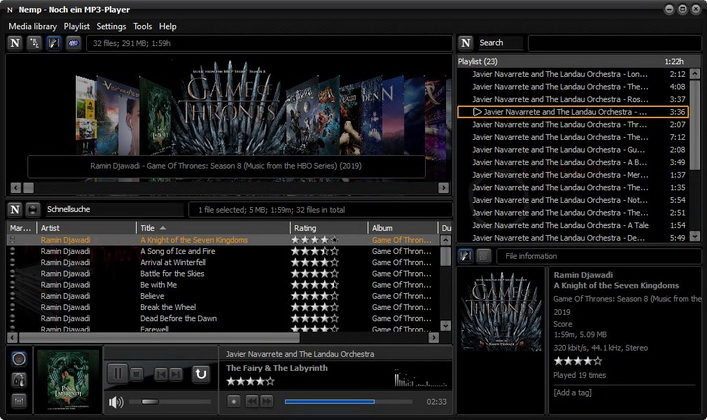
\includegraphics[width=0.8\textwidth]{v4_11.jpg}
\caption{New layout in Nemp 4.11}
\end{figure}

\begin{itemize}
\item The layout of the main window can now be modified using the \textbf{Form Designer}. The control panel of the player has been redesigned a bit:
	\begin{itemize}
		\item player and headphone controls share the same place
		\item display of the cover of the current title is smaller, but always visible
		\item display of the lyrics for the current title is dropped, but a display of the lyrics for the selected title in the playlist and media list 
		\item controls for effects and equalizer moved to separate window.
		\item removed the possibility to switch the scrolling title display between different informations
	\end{itemize}

\item Some changes and extensions to the skin system. Due to the new proportions of the window old skins may be incompatible and have to be adapted.
	\begin{itemize}
		\item Background graphics can be defined for individual areas, various options for alignment
		\item Bouncing bars in the taskbar preview removed. Instead more space for the title and a small progress bar.
		\item Use of some more skin colors also when the advanced skin system is used
	\end{itemize}
\item The sleep mode is no longer selected via a nested menu, but via a new dialog window.
\item Minor changes to the display in the playlist: The default note symbol is no longer displayed. For titles with cue sheets, the individual entries are displayed without quotes.
\item Deskband removed. It is still supported in principle, but since Nemp does not support Windows XP any more, and some other functions are not supported under XP, it is no longer included.
\end{itemize}

\subsection*{Version 4.10.0, July 2019}
\begin{itemize}
\item fixed the search for lyrics: new template, change to https
\item additional source for lyrics 
\item Switched from http to https where possible (scrobbling, search for cover, partially lyrics)
\item Upgrade to Delphi 10.3 Rio (Community Edition)
\item Various fixes and minor improvements on the GUI, especially for the progress indicator of longer lasting functions
\item Possible data loss in ID3 tags fixed when using automatic lyrics retrieval and getting extended tags
\item configurable maximum number of files for a Drag\&Drop operation (only manually in the Nemp.ini, value \texttt{[Allgemein]}-\texttt{maxDragFileCount})  

\end{itemize}

\subsection*{Version 4.9.2, January 2019}
\begin{itemize}
\item Fixed some issues with the displayed titles in the media list
\item setting how the display of \gf{marked files} works
\item Quicksearch saves now the 10 most recent search terms
\item Display of the current IP adresses in the settings dialog of the web server.
\end{itemize}

\subsection*{Version 4.9.1, August 2018}
\begin{itemize}
\item Performance of the display app for the G15 significantly improved and thereby greatly reduced the CPU load.
\end{itemize}


\subsection*{Version 4.9.0, August 2018}

\textbf{New features}
\begin{itemize}
\item Loading and saving the media library is more RAM-saving now
\item Preparation of the media library for accelerated searches is more RAM-saving now

\item option \gf{Ignore lyrics} to reduce storage problems with very (very) large music collections.
\item Logfile for the playlist: When was which track played
\item Option \gf{Delete missing files at startup} to delete missing files from the media library. If necessary, it will be executed again when a new drive is connected
\item Settings dialog: Button \gf{Scan now} for new or missing files
\end{itemize}

\textbf{Bugfixes}
\begin{itemize}
\item \gf{Cleanup / Remove missing files} removed always missing playlists, even from drives that are not currently connected
\item Possible deadlock at \gf{Clear Covercache} fixed
\end{itemize}

\subsection*{Version 4.8.0, March 2018}

\textbf{New features and changes}
\begin{itemize}
\item Possibility to mark files in the Media Library.
\item Support for SoundFont files for MIDI playback. (This is more like a bug fix.)
\item removed \gf{Extend Search} and \gf{Refine Search} from the detailed search window
\item command line parameter \texttt{/close}.

\end{itemize}


\subsection*{Version 4.7.1, November 2017}

\textbf{Bug fix}
\begin{itemize}
\item fixed an access violation when browsing playlists
\end{itemize}


\subsection*{Version 4.7.0, October 2017}

\textbf{New features}
\begin{itemize}
\item Search in the playlist. 
\item Option: In \gf{Repeat Title} playback mode, play only the current entry in a cuesheet and not the entire file.
\item Option: Weighted random play. Highly rated titles in the playlist are more likely to be selected than those with a low rating (or vice versa)
\item Option: Default cover configurable (again)
\end{itemize}

\textbf{Changes}
\begin{itemize}
\item Settings dialog revised. All options are always displayed. But some of these were sorted more sensibly and a little bit purified. Some old and very rarely used options have been dropped, some others have been added
\item Changes to some default settings that were relics of the past and caused confusion rather than clarity.
\end{itemize}

\textbf{Bug fixes}
\begin{itemize}
\item The keyboard display app now shows the current title when playing web radio, and not permanently the title that was active when the stream was started (if the channel is sending appropriate metadata)
\item Some webstreams seemed to block Nemp, fixed by a dedicated HTTP user agent instead of the bass.dll standard.
\end{itemize}


\subsection*{Version 4.6.3, December 2016}

\begin{itemize}
\item Fixed automatic lyric search (i. e. adapted to the new page layout of the source)
\item On web radio, the title in the playlist also changes automatically when the station transmits new metadata
\item Moving the window with cover, equalizer and effects control often led to a chaotic shift of the player window
\end{itemize}

\subsection*{Version 4.6.2, April 2013}

\begin{itemize}
\item Non-ASCII characters were displayed incorrectly on the web server, and the search for them did not work
\end{itemize}


\subsection*{Version 4.6.1, March 2013}

\begin{itemize}
\item Global switch-off option for the extended skin system, with default off for Windows XP

\item If the playlist is empty but a title is still running, it will now be played to the end when new files are inserted into the playlist. Exception: Playback and delete old playlist  

\item G15-App no longer reports an error at startup, if there is no G15.
  Usage can now also be (de-)activated in the Nemp settings dialog, not only in the app itself.
\end{itemize}

\subsection*{Version 4.6.0, February 2013}

\begin{itemize}
\item iTunes tags (m4a)
\item Walkman mode: Fluttering on low battery
\item New standard skin, including new logo
\item Settings dialog revised
\end{itemize}


\subsection*{Version 4.5.0, April 2012}
\begin{itemize}
\item Apev2 tags 
\item A-B repeat 
\item Skip silence at the end of a track 
\item Loading the library file in the background (faster startup)
\end{itemize}


\subsection*{Version 4.4.0, February 2012}

\begin{itemize}
\item Highly updated webserver: Themes, vote, usergroups, AJAX
\item New feature: Insert headphone track in playlist and play it from current position
\item Option \emph{Insert at the end of the bookmark list} changed to \emph{Insert after current title}. The one with the bookmark list is too confusing, and 
  especially in combination with the web server not understandable
\end{itemize}


\subsection*{Version 4.3.1, November 2011}

\begin{itemize}
\item After deleting the quick search (click on x) the preselection did not work anymore (except in the coverflow)
\end{itemize}

\subsection*{Version 4.3.0, November 2011}

%\textbf{New features and changes}
\begin{itemize}
\item Improved support for CD audio 
\item When dragging the position controller, the target time is displayed
\end{itemize}


\subsection*{Version 4.2.0, June 2011}
\begin{itemize}
\item Nemp Wizard, which asks for some important settings at first startup
\item Multimedia keys no longer by hook, but by hotkey
\item Setting \emph{Allow quick access to metadata}. This can be used to prevent unintentional changes to the ID3 tags (e.g. rating)
\end{itemize}

\subsection*{Version 4.1.0, April 2011}

%\textbf{New features and changes}
\begin{itemize}
\item Flac and Ogg tags (read and write)
\item support for the Logitech G15 display (through additional tool)
\item Copy\&Paste: Ctrl+Shift+C creates also a matching m3u list
\item \emph{Copy Playlist to USB-Stick} function. Optionally also with matching renaming files
\item Push-To-Talk Button (F8)
\item File Details: Editing additional tags (for the tag cloud)
\item File not found in \emph{last playlists}: offer \emph{delete entries}
\item If files are not tagged, select what should be displayed, e. g. path in the album column 
\item Nemp can now also be closed when the media library is performing an update.
\item Browsing in the Shoutcast database is disabled. The API has been changed and the Terms of Use exclude OpenSource.
\end{itemize}
 
\subsection*{Version 4.0.1, August 2010}

\begin{itemize}
\item Ratings were not saved to the ID3 tag if the Playback counter was set to 0
\end{itemize}

\begin{figure}[tbh]
\centering
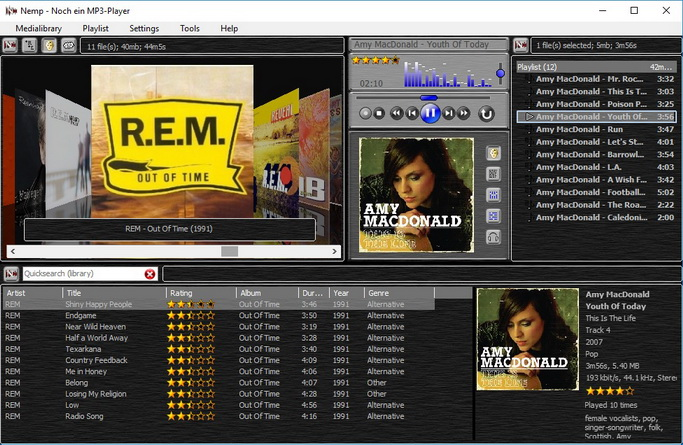
\includegraphics[width=0.7\textwidth]{v4_0.jpg}
\caption{Nemp as Open-Source}
\label{fig_4.0}
\end{figure}

\subsection*{Version 4.0.0, May-July 2010: Nemp becomes Open-Source}

\begin{itemize}
\item Change of the license from Freeware to Open Source: Nemp is now available under the GPL
\item Change of the development environment from Delphi 7 to Delphi 2009
\end{itemize}

\textbf{New Features}
\begin{itemize}
\item New Coverflow
\item Automatic download of covers from the Internet
\item Added browse mode \emph{tag cloud}.
\item Lyricsearch on the web works again
\item Edit file information directly in the main window. Start editing by double-clicking or F2, change the rating with a single click
\item Automatic adjustment of the rating for frequently played files. The change in the rating depends on the play counter (in the case of often heard titles, the rating changes less strongly)
\item Windows7 support extended: Customized taskbar preview window, taskbar volume buttons, progress bar for longer actions in the taskbar
\item Direct playback from the media library possible without changing the playlist
\item Prebook list in the playlist. Playback sequence can be changed using the numeric keys. 
\item Playlist history
\item Party Mode: Larger buttons with reduced function to avoid unintentional incorrect entries.
\item Web radio management improved. Sorting option for the web radio stations in the media library, export of the web radio stations as pls-file
\item Smarter resizing of components when resizing the main window
\item Headphone control integrated in the main window: easy insertion of the current headphone title into the playlist
\end{itemize}

\textbf{Changes}
\begin{itemize}
\item Removed skin editor from main program
\item \emph{Quick search} revised. Everything is always searched, not just the current list. Hits from this list are displayed first.
\end{itemize}

\subsection*{Version 3.3.4, November 2009}

\begin{itemize}
\item Under certain circumstances, the playlist played only one song and then stopped
\end{itemize}


\subsection*{Version 3.3.3, August 2009}

\begin{itemize}
\item Automatic lyrics search removed. LyricWiki had to shut down the API due to pressure from record companies

\item Missing files in the playlist were not skipped, respectively  playback stopped automatically afterwards
\end{itemize}


\subsection*{Version 3.3.2, July 2009}

\begin{itemize}
\item Fixed various errors when booting from CD/DVD or other write-protected media
\item The function \emph{Remove played title from playlist} did not work
\item Disabling automatic update search did not work
\end{itemize}


\subsection*{Version 3.3.1, April 2009}

\begin{itemize}
\item Editing ID3 tags resulted in inconsistencies in the media library (double files) or a total player crash.
\end{itemize}


\subsection*{Version 3.3.0, March 2009}

\textbf{New features}
\begin{itemize}
\item LastFM Scrobble. Played songs are stored in the LastFM user profile.
\item Updater function, i.e. automatic notification of new versions
\item Web radio recording with cut by time/file size
\item If a new drive with a monitored directory is connected, scanning for new files may start afterwards if necessary
\item Rudimentary Windows7 support (task bar buttons)
\end{itemize}

\textbf{Changes}
\begin{itemize}
\item Settings dialog revised
\item About dialog revised
\item File type registration extended, e.g. display of the currently registered file types on Nemp
\end{itemize}

\textbf{Bug fixes}
\begin{itemize}
\item The volume keys on multimedia keyboards didn't work as expected
\item The volume control on jingles was defective
\item The playlist files had problems with very long file names
\item Tags in Lossless WMA files were not retrieved
\end{itemize}



\subsection*{Version 3.2.1, January 2009}
\begin{itemize}
\item If no media library was loaded, the deskband did not work properly
\item Access violations occurred after executing the function \gf{Delete missing files} during quick search
\item In the German version, some album or artist names were displayed incorrectly in the coverflow, e.g. \emph{Pos1} if the album is called \emph{Home}
\end{itemize}


\subsection*{Version 3.2.0, December 2008}
\textbf{New features and changes}
\begin{itemize}
\item A very special hidden feature ;-)
\item In Coverflow, the \gf{All Files} cover can be personalized, i. e. 1-8 random covers from the media library are used for this purpose
\end{itemize}

\textbf{Bug fixes}
\begin{itemize}
\item Fixed a bug in MP3FileUtils that may have cut off the last character.
\end{itemize}


\subsection*{Version 3.1.0, November 2008}

\textbf{New features}
\begin{itemize}

\item Significantly faster search in the media library. 
  This means: The search via the quick search runs in real time during typing - optionally even with error tolerance, an error-tolerant search is preset when pressing the Enter key
\item Significantly improved download of lyrics. This means faster, more reliable and simpler. The additional program EvilLyrics is no longer needed.
\item Integration of playlists into the media library. Playlist files are also taken into account when searching the hard disks for music files. These can be inserted completely into the current playlist via the preselection or via the lower title list only partially.
\item Significantly improved support of Webradio. Search in the Shoutcast database and bookmark management.
\item Integrated web server added. In addition, it is possible to exchange your own music collection with friends - limited to the LAN or worldwide. Optionally, the player can also be controlled via this. On the other hand, a normal web browser is sufficient. The previous Remote Nemp, which only worked very moderately, was stamped.
\item Ratings of individual titles
\item Cover images in PNG format (also in ID3 tag)
\item FLAC metadata
\item Playback mode No repeat added, i.e. playback does not restart when the playlist is finished.
\item Binary playlist format added, which can store additional information and accelerates the loading process, since this information no longer has to be retrieved individually from the mp3 files.
\end{itemize}

\textbf{Changes}
\begin{itemize}
\item Improved handling of wrong drives. This means that Nemp notices whether the drive E: from the last session corresponds to the current E: and initiates appropriate actions if necessary. This also works with drives that are connected afterwards (i.e. while Nemp is running) 
\item Redesigned detail window. Editing ID3 tags should now be more intuitive. Additional information is displayed (e.g. URL and copyright information)
\item Click on the Next button to jump (optional) to the next entry in the cue sheet only
\item More choice for automatic shutdown of the system, clearer layout
\item The Play/Pause, Stop and Playback mode buttons now have a pop-up menu
\item If Nemp is not terminated correctly, no warning message will be issued at the next startup. The automatically backed up backup playlist is loaded.
\item Inserting many files from the media library into the playlist is now much faster (using the menu items Drag\&Drop, Copy\&Paste is only possible with max. 500 files possible)
\end{itemize}

\textbf{Bug fixes}
\begin{itemize}
\item Under some circumstances an error occurred, when recording web radio a file name is too long.
\item ID3 tags of mp3 files from jamendo.com were often read incorrectly
\item Track numbers were often not retrieved from WMA files
\item When playing backwards with increased speed, the Mickey Mouse effect always occurred, even if this was switched off in the settings.
\end{itemize}


\subsection*{Version 3.0.3, June 2008}
\begin{itemize}
\item Cue lists had a problem with the last entry in the list
\item In cue lists, the display of the current entry sometimes didn't match
\item Changing the options changed the playback to the headphone volume
\item In 3.0.2, the error that the language was reset to English appeared again if no language was explicitly selected and the settings dialog was called.
\end{itemize}


\subsection*{Version 3.0.2, May 2008}

\textbf{Changes}
\begin{itemize}
\item update of the bass.dll from version 2.3 to 2.4, possibly installed add-ons must also be updated
\item Added settings for playback that can fix problems with distorted playback on some systems.
\end{itemize}

\textbf{Bug fixes}
\begin{itemize}
\item The quick search for the empty string was not really quick.
\item The first entry in the playlist could not be selected via the tray menu.
\item Updating the cover in the media library worked partially not correctly.
\item Getting lyrics caused a bug cascade.
\end{itemize}

\subsection*{Version 3.0.1, November 2007}

\begin{itemize}
\item If no language has been explicitly set, the first time the options dialog was called the language changed to English, even if German was correctly recognized at startup
\item The deskband didn't display the commercial and (\&) correctly
\end{itemize}

\begin{figure}[tbh]
\centering
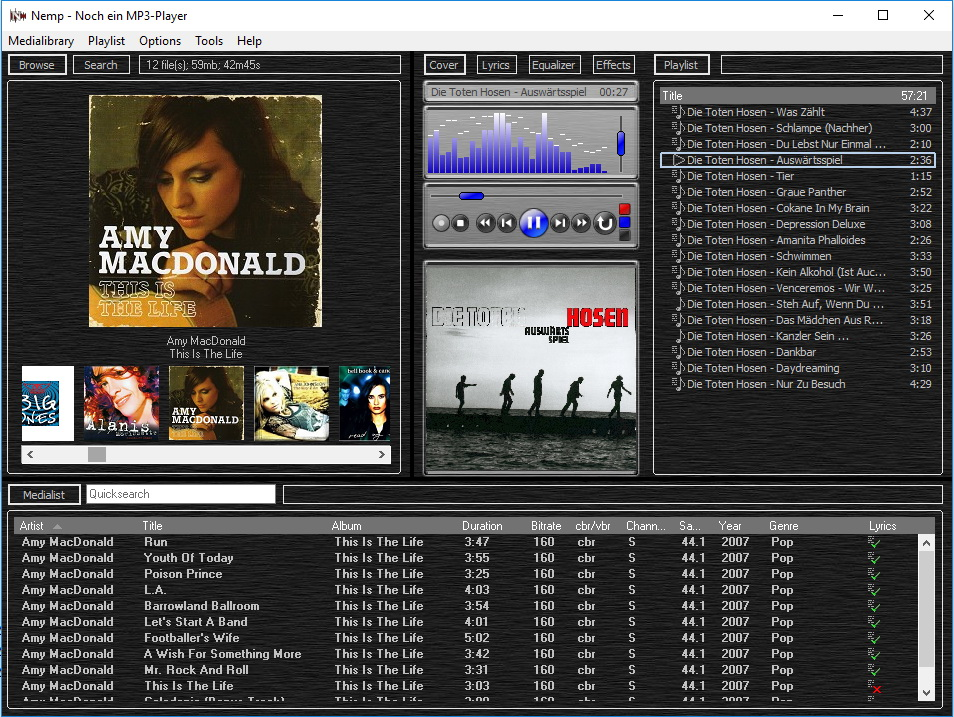
\includegraphics[width=0.7\textwidth]{v3_0.jpg}
\caption{Nemp after the first general overhaul}
\label{fig_3.0}
\end{figure}


\subsection*{Version 3.0.0, October 2007: Almost completely reworked}

\textbf{New features}
\begin{itemize}
\item API included. Nemp can be controlled via third-party programs: controlling the player, displaying the playlist, searching in the media library and adding search hits to the playlist 
\item As an example application for the API: a deskband embedding itself in the taskbar 
\item Remote-Nemp: Connect to other Nemp (via LAN or the Internet), browse the foreign media library, download individual titles from friends, add-on tools to control the other Nemp are possible (documentation will follow later) 
\item Coverflow
\item Random playlists. Parameters are possible: genres (with configurable preselections), time period, number of titles
\item Cue sheets
\item Birthday mode: Specify the date and time, select the song, and the song will play automatically at that time. Optionally, a countdown can be played beforehand. The countdown is automatically started before the start of the countdown
\item multilanguage system. Almost arbitrarily expandable. Translation files can be created by yourself and easily integrated. If available, the system will automatically select the appropriate language - otherwise English
\item Recording of web radio with automatic track splitting. Configurable file naming, automatic addition of ID3 tags
\item The current position in the track is saved at the end of the track and restored the next time it is started.
\item Support of m3u8 playlists for correct saving of Unicode playlists
\end{itemize}

\textbf{Improved features}
\begin{itemize}
\item Skin system improved. No more flickering when enlarging the windows. Position and size of the control buttons variable. Self-configurable hover effects for the buttons 
\item Sleep mode alternatives: Nemp exit, suspend, hibernate, shutdown
\item Tray-Popup contains parts of the playlist
\item More comfort in the media library. While searching for new files, the library is not locked for browsing and searching. Search hits can be dragged into the playlist using drag\&drop, even if the search is still running. Selected folders can be monitored, i.e. new files are automatically integrated into the library the next time they are started.
\item Improved quick search. The search term entered is divided into individual words and these are searched for individually. Contiguous words can be stapled by quotation marks.
\item Settings dialog revised. 
\item Configurable Hotkeys
\item Enhanced Equalizer
\item Jingle volume configurable
\item Any files are accepted for the playlist via Drag\&Drop
\end{itemize}

\textbf{Changes}
\begin{itemize}
\item XP/nonXP version changed. It no longer depends on the file name, but on the folder in which Nemp is located.
\end{itemize}

\textbf{Internal stuff}
\begin{itemize}
\item Code of the player almost completely rewritten
\item Code for managing the playlist almost completely rewritten
\item Code for media bib management almost completely rewritten
\end{itemize}

 
\subsection*{Version 2.5d, November 2006}
\begin{itemize}
\item Several minor bug fixes
\end{itemize}

\subsection*{Version 2.5c, Oktober 2006}
\begin{itemize}
\item Random playback improved (avoid repeating a song after a short time)
\item Option Play now 
\item The media list is now loaded in the background at startup
 \end{itemize}


\subsection*{Version 2.5b, September 2006}
\begin{itemize}
\item Several minor bug fixes
\end{itemize}

\subsection*{Version 2.5a, September 2006}
\begin{itemize}
\item Skins are now collected in the \verb+\Skins\+ subfolder. Old skins must be moved there
\item Sleep mode: Choose between shutting down Windows and quitting Nemp 
\item Skin setting: Align wallpaper on desktop or middle part of the player
\end{itemize}

\begin{figure}[tbh]
\centering
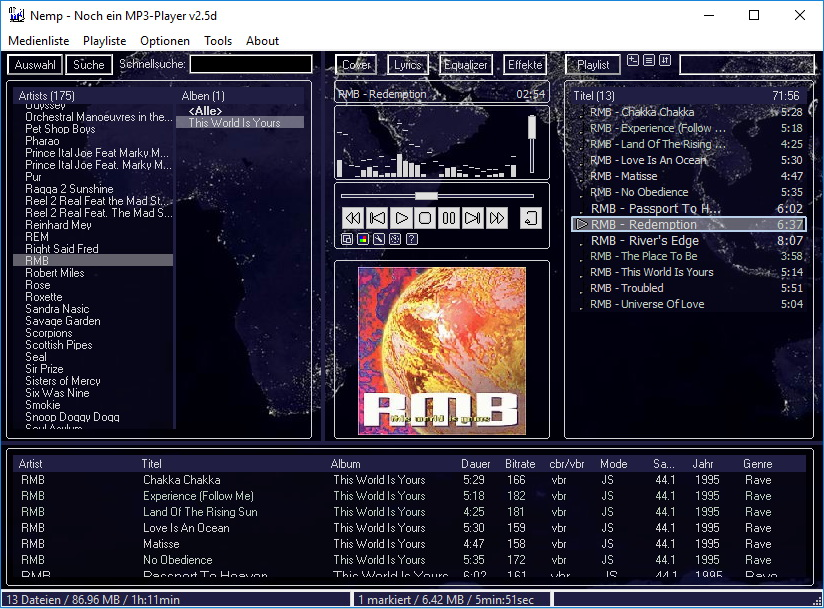
\includegraphics[width=0.7\textwidth]{v2_5.jpg}
\caption{Nemp vor der ersten General�berholung}
\label{fig_2.5}
\end{figure}

\subsection*{Version 2.5, September 2006}

\textbf{New features}

\begin{itemize}
\item Extensive Unicode support. 
\item Variable Preselection for the media list. Not only Artist-Album, but variable (artist, album, genre, year, folder)
\item Variable window design: Compact mode or single window
\item Registration of the data types that Nemp knows and entries in the context menus of folders: Play/insert in Nemp 
\item Random playback of the playlist
\item Control of the files played back in the headphones
\item Sleep mode
\end{itemize}

\textbf{Changes}
\begin{itemize}
\item Drag\&Drop from the media list to the playlist is also successful if the downloaded files are not available
\item Dragging of more than 500 files is prevented
\item Searching for new files now uses SearchTools and is therefore somewhat faster
\item Unknown genres from the ID3v2 tag are now saved in the media list
\end{itemize}

\textbf{Bug fixes}
\begin{itemize}
\item pressure on [DEL] in the search entries led to a removal of an entry in the media list or even to a crash of the program.
\item When fading was activated, it may happen that a click on Pause was ignored
  \end{itemize}


\subsection*{Version 2.4, June 2006}

\begin{itemize}
\item PlugIn system for easy support of other file formats.
\item Webradio (ShoutCast/Icecast)
\item Quick search
\item Switch from bass2.2 to bass2.3
\item Global Hotkeys
\item StayOnTop of the player
\end{itemize}

\subsection*{Version 2.3, May 2006}

\begin{itemize}
\item Extensive skin system added, including matching editor
\item 4 different display modes - from complete to minimal
\item Nemp now understands parameters - so you can set it up as a standard application for mp3 files
\item Only one instance of Nemp possible (can be disabled)
\item Improved support for wma files
\item Equalizer Presets 
\item Effect: change playback speed with or without mickey mouse effect 
\item Reverse Playback
\item Jingles
\item Drag\&Drop of artists and albums 
\item Playback of various other file types. Among other things mod, xm, aiff
\item Export media list as .csv
\item Improved support for m3u playlists
\end{itemize}

\subsection*{Version 2.2, March 2006}
\textbf{New features and changes}
\begin{itemize}
\item Enhanced support for multimedia keyboards by using a hook
\item Equalizer  
\item Effects (speed, echo, reverb) 
\item PLS playlists
\item Clicking on ID3v1-Save or ID3v2-Save now also causes saving of the change in the other tag version
\end{itemize}

\textbf{Bug fixes}
\begin{itemize}
\item Drop in the playlist from Windows Explorer caused an unnecessary rebuild of the media list
\item No wma files could be played in the headset
\item Better suppport for m3u playlists
\end{itemize}


\begin{figure}[tbh]
\centering
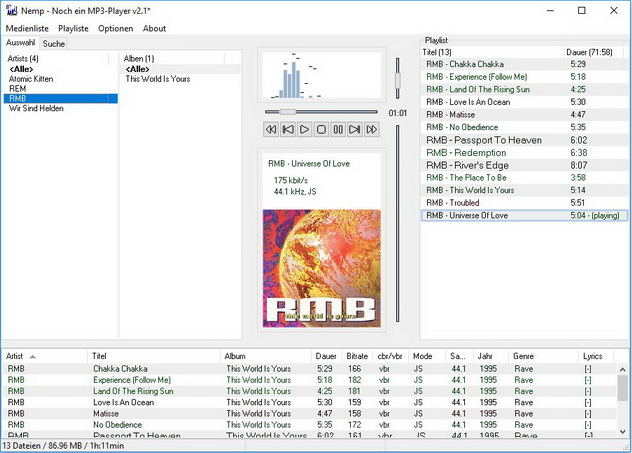
\includegraphics[width=0.7\textwidth]{v2_1.jpg}
\caption{The first Nemp}
\label{fig_2.1}
\end{figure}


\subsection*{Version 2.1, February 2006: Nemp becomes an mp3 player}

\textbf{Major Updates/Changes: }
\begin{itemize}
\item Internal Player added
\item New icon and renaming of \emph{Gausis MP3 Verwaltung} to \emph{Nemp - Noch ein MP3-Player}
\item Direct search in the media list simplified
\item Classification into predefined categories such as albums, samplers, soundtracks removed
\item Automatically save/load media list and playlist on exit and startup
\item Modification of the system to allow storage independent of the drive. This means that changing the drive letter for multiple partitions is (almost) no problem anymore
\item Search in separate thread outsourced
\item \emph{Get Lyrics with EvilLyrics} 
\end{itemize}


\textbf{Minor Updates/Changes}
\begin{itemize}
\item Display of the media list slightly changed
\item Winamp connection further loosened. With your own player it doesn't make sense to monitor the Winamp status anymore
\end{itemize}


\subsection*{Version 2.0, September 2005}
\textbf{Major Updates/Changes}
\begin{itemize}
\item More detailed display of file details
\item Complete editing of id3v1/id3v1.1 tags
\item Extensive editing of id3v2Tag, including pictures and lyrics 
\item Lyric search added - you can search for a line in the lyrics of the song
\item Search by date/genre
\item Fuzzy search
\item Size of the .gmp files reduced by almost 50\%. 
\item Storage of comments in alternative data streams (ADS) under NTFS removed - the id3v2 tags are now available for this purpose
\end{itemize}

\textbf{Minor Updates/Changes}
\begin{itemize}
\item Reading the information year and genre from the ID3 tags
\item Removed remote control for Winamp
\end{itemize}


\subsection*{Version 1.1, January 2005}
\begin{itemize}
\item Replacement of the StringGrid component with VirtualTreeView - resulting in much nicer operation.
\item Search history
\item Simple acceleration of search function
\end{itemize}

\subsection*{Version 1.0, first release, January 2005}
\begin{figure}[tbh]
\centering
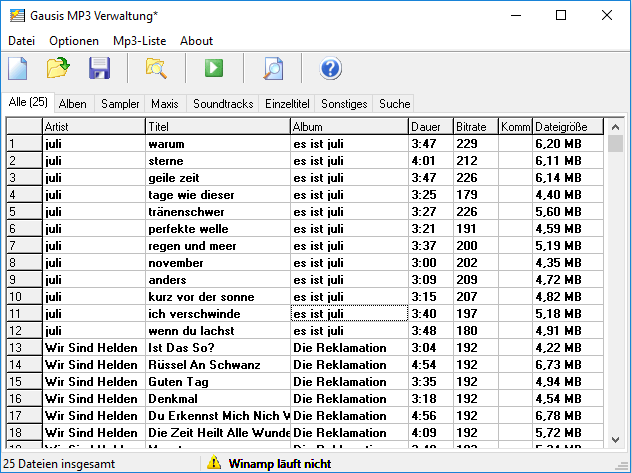
\includegraphics[width=0.8\textwidth]{v1_0.png}
\caption{Gausis Mp3-Verwaltung 1.0, from which Nemp should emerge later on}
\label{fig_1.0}
\end{figure}


\end{document}




\subsection*{Neu in Version 4.6}
\begin{itemize}
\item Unterst�tzung f�r iTunes-Tags 
\item Schnellerer Start der Wiedergabe (besonders bei Dateien auf Netzwerk-Laufwerken) 
\item Walkman-Modus (Wiedergabe leiert bei schwachem Akku) 
\item �berarbeiteter Einstellungs-Dialog 
\item Kleinere �nderungen am GUI 
\item Diverse Bugfixes (*.cda in Medienbibliothek, Playnext bei sehr kurzen Titeln) 
\end{itemize}

\subsection*{Neu in Version 4.5}
\begin{itemize}
\item Unterst�tzung von Apev2-Tags 
\item A-B-Wiederholung 
\item �berspringen von Stille am Ende eines Titels 
\item Auswerten der Meta-Information CD-Nr. bzw. Part of a Set bei Multi-CD-Alben 
\item Optionen: Kein Splashscreen, Wechseln zu neu eingef�gtem Titel (bei Doppleklick im Explorer bei bereits laufendem Player) 
\item Laden der Bibliotheks-Datei im Hintergrund (schnellerer Start) 
\item Diverse �nderungen an der GUI
\item Diverse Bugfixes (Sortieren nach Dateiname/Ordner, Kein Wiederholen, Trackermodul-Dateien) 
\end{itemize}

\subsection*{Neu in Version 4.4 (Auszug)}
\begin{itemize}
\item Stark �berarbeiteter Webserver: Positionsanzeige und Spulen im aktuellen Titel, Lautst�rkeregelung, Sortieren und L�schen von Titeln in der Playlist, St�bern in der Medienbibliothek nach Interpret, Album oder Genre, optionale Unterteilung zwischen usern und Administratoren 
\item Der Webserver ist �ber Themes (relativ) leicht den eigenen W�nschen entsprechend anpassbar.  
\item Neue Funktion: Kopfh�rer-Titel in Playlist einf�gen und ab aktueller Position abspielen 
\item �nderung: Drag\& Drop in die Playlist f�gt die Dateien hinter den markierten Titel ein, nicht mehr davor 
\end{itemize}

\subsection*{Neu in Version 4.3 (Auszug)}
\begin{itemize}
\item Bessere Unterst�tzung von CD-Audio
\item Funktion Medienbibliothek aufr�umen erweitert (d.h. Auswahl, ob fehlenden Dateien auf nicht verf�gbaren Laufwerken doch behalten werden sollen) 
\item neue bassFX-Version. dann klappts auch mit Windows 8 
\item Umstellung auf die neue Scrobble-API 
\end{itemize}

\subsection*{Neu in Version 4.2 (Auszug)}
\begin{itemize}
\item Multimediatasten sollten jetzt endlich vern�nftig funktionieren 
\item Strg+V f�gt Dateien in der Playlist jetzt an der markierten Stelle ein 
\item Wizard hinzugef�gt, der einige grundlegende Einstellungen abfragt 
\item Alles, was im Hintergrund passiert und Musikdateien �ndert oder neue Dateien erstellt (mit Ausnahme der Konfigurationsdateien, Medienbibliothek, Playlist usw. im Daten-Verzeichnis), ist jetzt Opt-In, d.h. es muss explizit erlaubt werden. Genau diese Dinge fragt der Wizard ab. 
\end{itemize}

\subsection*{Neu in Version 4.1 (Auszug)}
\begin{itemize}
\item Unterst�tzung von Ogg- und Flac-Tags 
\item Kopieren der Playlist inklusiver passender m3u-Datei durch Strg+Shift+C 
\item Funktion Playlist in Verzeichnis kopieren (z.B. auf einen USB-Stick) mit Umbenennung der Dateien 
\item Push-To-Talk durch F8 (�hnlich der Jingles) 
\item Unterst�tzung f�r das Display der Logitech G15 (andere Tastaturen k�nnen nachger�stet werden, wenn das jemand machen m�chte) 
\end{itemize}

\subsection*{Neu in Version 4.0 (Auszug)}
\begin{itemize}
\item Sch�nerer Coverflow mit automatischem Cover-Download 
\item Browsemodus Tagwolke
\item Einfachere Bearbeitung der mp3-Dateien 
\item Unterst�tzung f�r Windows 7 
\item Partymodus mit vergr��erter Ansicht und reduzierten Funktionen 
\item Vormerk-Liste f�r die Playlist 
\item ... 
\end{itemize}



